\documentclass[12pt, a4paper]{article}
\usepackage[default]{lato}
\usepackage[T1]{fontenc}
\usepackage[polish]{babel}
\usepackage{polski}
\usepackage[left = 2cm,right = 2cm,top = 2cm,bottom = 2.5cm]{geometry}
\usepackage{indentfirst}
\usepackage[dvipsnames]{xcolor}
\usepackage{amsmath}
\usepackage{amsfonts}
\usepackage{float}
\usepackage{graphicx}
\usepackage{fancyhdr}
\usepackage{multicol}
\usepackage{multirow}
\usepackage[RPvoltages]{circuitikz}
\usepackage{hyperref}
\usepackage{enumitem}
\usepackage{titlesec}
\usepackage{chngcntr}

% make new section on new page
\newcommand{\subsectionbreak}{\clearpage}
\newcommand{\sectionbreak}{\clearpage}

% section title before number
\titleformat{\section}{\center\normalfont\Large\bfseries}{}{0em}{}

% section title before number
\titleformat{\subsection}{\normalfont\large\bfseries}{}{0em}{}

% subsection numbering without section number
\renewcommand{\thesubsection}{\arabic{subsection}}

% reset equation numer each section and subsection
\counterwithin*{equation}{section}
\counterwithin*{equation}{subsection}

% also print numbers of section and subsections with equations numbers
\renewcommand{\theequation}{\arabic{section}.\arabic{subsection}.\arabic{equation}}

% set first section counter to 0
\setcounter{section}{-1}

\hypersetup{
 colorlinks=true,
 linkcolor=blue,
 filecolor=magenta,
 urlcolor=cyan,
}

\newcommand{\makeTilte}[4]
{\begin{titlepage}
 \newcommand{\HRule}{\rule{\linewidth}{0.5mm}}
 \center
 
\includegraphics[scale=.7]{./images/PWr.png} \\[1cm]
 {\textbf{\Large {#1}}}\\[0.5cm]
 {\textbf{\large {#2}}}\\[0.5cm]
 \HRule \\[0.5cm]
 {\huge \bfseries {#3}} \\[0.2cm]
 \HRule \\[1.5cm]
 \begin{minipage}{0.5\textwidth}
  \begin{center}
   \large \textbf{{#4}}\\[0.5cm]
   \emph{Automatyka i Robotyka,\\
    Wydział Elektroniki,\\
    Politechnika Wrocławska}
  \end{center}
 \end{minipage} \\[2cm]
 \vspace*{4.5cm}
 {\large \today} \\[2cm]
 \vfill
\end{titlepage}
\pagestyle{empty}
\tableofcontents
\newpage
\pagestyle{fancy}
\fancyhf{}
\headheight = 30pt
\cfoot{\textcolor{Gray}{{#1} - {#3}}}
\lhead{\leftmark}
\rhead{{#4}\\Strona \thepage}
\renewcommand{\headrulewidth}{1.5pt}
\renewcommand{\footrulewidth}{0.5pt}}

\newcommand{\slimHeader}[2]
{\pagestyle{fancy}
\fancyhf{}
\headheight = 60pt
\rhead
{{#1} \\
{#2} \\
Strona \thepage}
\renewcommand{\headrulewidth}{1.5pt}}


\begin{document}
\makeTilte
{Podstawy elektrotechniki i elektroniki}
{Wykładowca - dr inż. Zbigniew Świętach}
{Opracowanie ćwiczeń}
{Jakub Kozłowicz, Maciej Kaniewski}

%---------------------------- LISTA 1 -----------------------------------------
\section{Od autorów}
\vspace*{2cm}
Opracowanie to powstało w roku akademickim 2020/2021, w semestrze zimowym.
Wartość merytoryczną jak i wiele rysunków przygotował Maciej Kaniewski.
Złożył i opracował Jakub Kozłowicz.

Jak wiemy z roku na rok zadania od prowadzących się zmieniają, jednak opracowanie
to zawiera opis wszystkich metod i pozwala zrozumieć jak rozwiązywać takie zadania.
\vspace*{2cm}
\begin{flushright}
  \textit{Pozdrownienia\\Rocznik 2k19.}
\end{flushright}

\section{Lista 1}
% Zadanie 1
\subsection{Zadanie 1}
\textbf{Wyznaczyć wartości średnią i skuteczną następujących sygnałów okresowych.
  Wartość średnia $F_{sr} = \dfrac{1}{T}\int\limits_{t_0}^{t_0+t}f(t)dt$,
  wartość skuteczna $F_{sk} = \sqrt{\dfrac{1}{T}\int\limits_{t_0}^{t_0+t}f^2(t)dt}$.}

% Zadanie 2
\subsection{Zadanie 2}
\textbf{Wyznaczyć rezystancję wypadkową następujących dwójników.}
\begin{figure}[H]
  \centering
  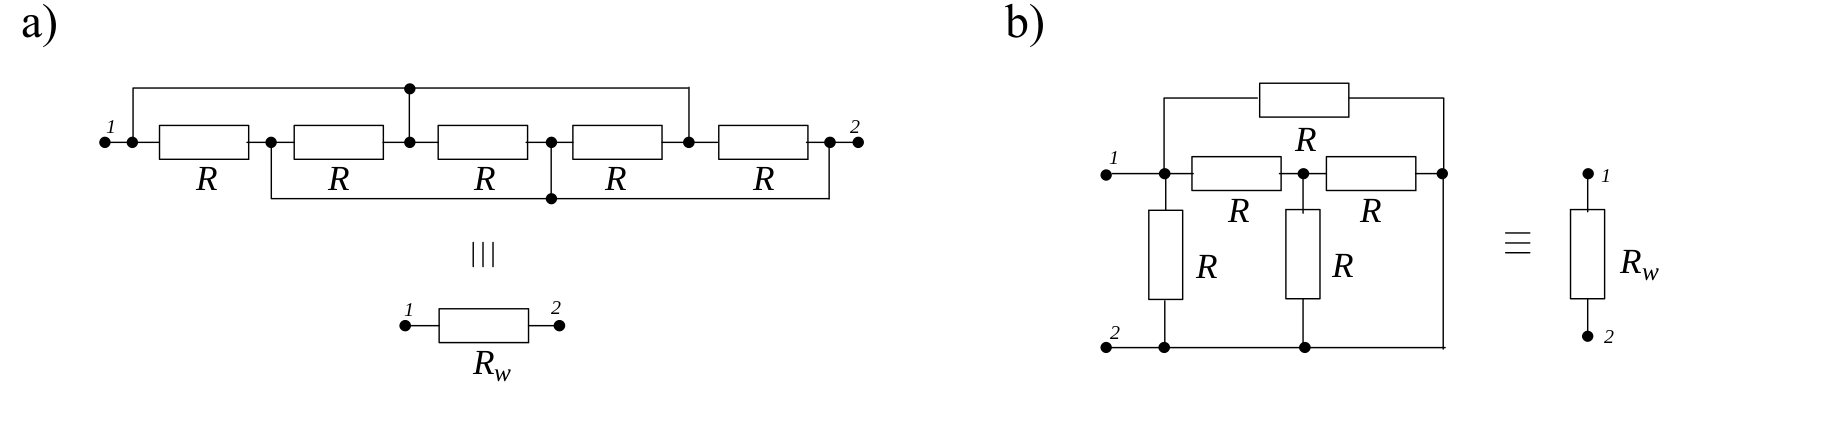
\includegraphics[width = \textwidth]{./images/Lista_1/Zadanie_2.png}
\end{figure}
\paragraph{Rozwiązanie}
\begin{enumerate}[label=\alph*)]
  \item Wszystkie te rezystory są połączone równolegle, ponieważ znajdują się
        między dwoma tymi samymi potencjałami 1 i 2.
        \begin{figure}[H]
          \centering
          \includegraphics[width = 0.7\textwidth]{./images/Lista_1/Zadanie2_rozwiązanie.png}
        \end{figure}
        $$
          \frac{1}{R_w} = \frac{1}{R} + \frac{1}{R} + \frac{1}{R} + \frac{1}{R} + \frac{1}{R}
        $$
        $$
          \frac{1}{R_w} = \frac{5}{R}
        $$
        $$
          R_w = \frac{1}{5}R
        $$
  \item Przekształćmy ten obwód do bardziej przystępnej postaci.
        \begin{figure}[H]
          \centering
          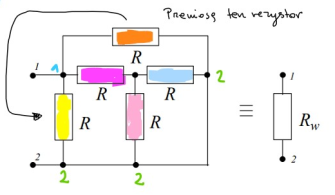
\includegraphics[width = 0.3\textwidth]{./images/Lista_1/Zadanie2b_1.png}
          $ \Rightarrow $
          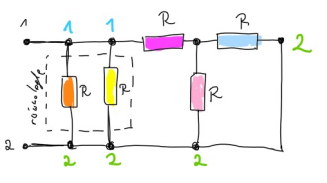
\includegraphics[width = 0.3\textwidth]{./images/Lista_1/Zadanie2b_2.png}
          $ \Rightarrow $
          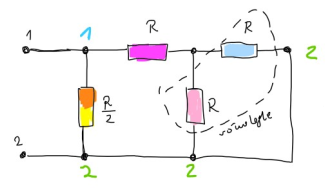
\includegraphics[width = 0.3\textwidth]{./images/Lista_1/Zadanie2b_3.png}
        \end{figure}
        \begin{figure}[H]
          \centering
          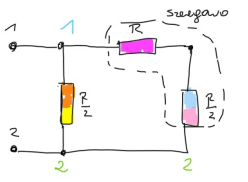
\includegraphics[width = 0.3\textwidth]{./images/Lista_1/Zadanie2b_4.png}
          $ \Rightarrow $
          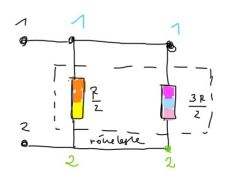
\includegraphics[width = 0.3\textwidth]{./images/Lista_1/Zadanie2b_5.png}
        \end{figure}
        $$
          \frac{1}{R_w} = \frac{1}{\dfrac{R}{2}} + \frac{1}{\dfrac{3R}{2}}
        $$
        $$
          \frac{1}{R_w} = \frac{2}{R} + \frac{2}{3R}
        $$
        $$
          \frac{1}{R_w} = \frac{6}{3R} + \frac{2}{3R}
        $$
        $$
          8R_w = 3R
        $$
        $$
          R_w = \frac{3}{8}R
        $$
\end{enumerate}
% Zadanie 3
\subsection{Zadanie 3}
\textbf{Wyznaczyć i narysować napięcie u(t) dla zadanego prądu i(t) płynącego przez dwójnik.}
\begin{figure}[H]
  \centering
  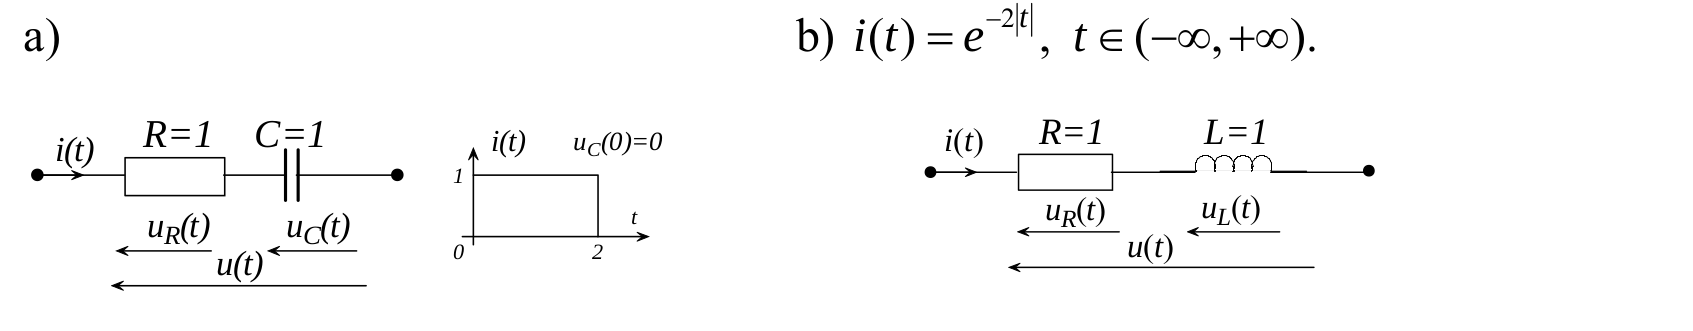
\includegraphics[width = \textwidth]{./images/Lista_1/Zadanie_3.png}
\end{figure}
\paragraph{Rozwiązanie}
\begin{enumerate}[label=\alph*)]
  \item Jako, że elementy są połączone szeregowo to końcowe napięcie będzie
        sumą napięć na rezystorze i kondensatorze
        $$
          u = u_R + u_C.
        $$
        Wyznaczmy teraz napięcie na rezystorze i prąd na kondensatorze
        \begin{equation}\label{1.3_rezystor1}
          u_R(t) = Ri(t),
        \end{equation}
        \begin{equation}\label{1.3_kondensator}
          i(t) = C\frac{du_c(t)}{dt}.
        \end{equation}
        Suma równania \ref{1.3_rezystor1} i scałkowanego równania \ref{1.3_kondensator}
        da nam napięcie całkowite wyrażone wzorem
        \begin{equation}\label{1.3_napiecie1}
          u(t) = Ri(t) + \frac{1}{C}\int\limits_{-\infty}^t i(\tau) d\tau.
        \end{equation}

        \begin{itemize}
          \item \textbf{t < 0}
                $$
                  i(t) = 0 \quad \Rightarrow \quad u(t) = 0
                $$
          \item \textbf{0 < t < 2}
                $$
                  u(t) = Ri(t) + \frac{1}{C}\int\limits_{-\infty}^t i(\tau) d\tau
                  \quad \Rightarrow \quad
                  u(t) = Ri(t) + u_C(0)+\frac{1}{C}\int\limits_0^t i(\tau) d\tau
                $$
                $$
                  u_C(0) = \frac{1}{C}\int\limits_{-\infty}^0 i(\tau) d\tau = 0
                $$
                $$
                  u(t) = 1 + 0 +\int\limits_{0}^t 1 d\tau =  1+t
                $$
          \item \textbf{t > 2}
                $$
                  u(t) = Ri(t) + \frac{1}{C}\int\limits_{-\infty}^t i(\tau) d\tau
                  \quad \Rightarrow \quad
                  u(t) = Ri(t) + u_C(2)+\frac{1}{C}\int\limits_2^t i(\tau) d\tau
                $$
                $$
                  u_C(2) = \int\limits_{0}^t 1 d\tau = \int\limits_{0}^2 1 d\tau = 2
                $$
                $$
                  u(t) = 0 + 2 +\int\limits_{2}^t 0 d\tau =  2
                $$
        \end{itemize}
        \textit{Uwaga, brak ciągłości napięcia $u(t)$ w punktach $t=0$ i $t=2$.}
  \item Jako, że elementy są połączone szeregowo to końcowe napięcie będzie
        sumą napięć na rezystorze i induktorze
        $$
          u = u_R + u_L.
        $$
        Wyznaczmy teraz napięcie na rezytorze i induktorze
        \begin{equation}\label{1.3_rezystor2}
          u_R(t) = Ri(t),
        \end{equation}
        \begin{equation}\label{1.3_induktor}
          u_L(t) = L\frac{di(t)}{dt}.
        \end{equation}
        Suma równania \ref{1.3_rezystor2} i  równania \ref{1.3_induktor}
        da nam napięcie całkowite wyrażone wzorem
        \begin{equation}\label{1.3_napiecie2}
          u(t) = Ri(t) + L\frac{di(t)}{dt}.
        \end{equation}

        \begin{itemize}
          \item \textbf{t < 0}
                $$
                  u(t) = Ri(t) + L\frac{di(t)}{dt}
                  \quad \Rightarrow \quad
                  u(t) = e^{2t}+\frac{de^{2t}}{dt} = e^{2t} + 2e^{2t} = 3e^{2t}
                $$
          \item \textbf{t > 0}
                $$
                  u(t) = Ri(t) + L\frac{di(t)}{dt}
                  \quad \Rightarrow \quad
                  u(t) = e^{-2t}+\frac{de^{-2t}}{dt} = e^{-2t} - 2e^{2t} = -e^{-2t}
                $$
        \end{itemize}
        \textit{Uwaga, brak ciągłości napięcia $u(t)$ w punkcie $t=0$.}
\end{enumerate}
% Zadanie 4
\subsection{Zadanie 4}
\textbf{Wykazać równoważność rzeczywistych źródeł napięciowego i prądowego.}
\begin{figure}[H]
  \centering
  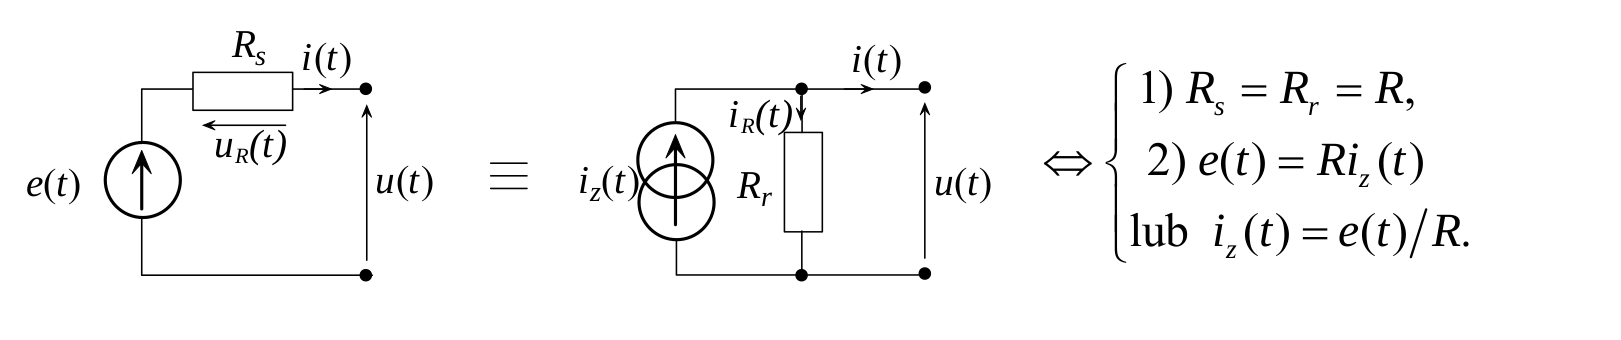
\includegraphics[width = \textwidth]{./images/Lista_1/Zadanie_4.png}
\end{figure}

Obwody są równoważne jeżeli w każdych warunkach pracy prądy i napięcia na zaciskach
zewnętrznych są jednakowe w obydwu układach.

\paragraph{Rozwiązanie}
\begin{itemize}
  \item \textbf{Rzeczywiste źródło napięcia}
        \begin{itemize}
          \item Rozwarcie
                $$
                  i(t) = 0 \: \Rightarrow \: u(t) = e(t)
                $$
          \item Zwarcie
                $$
                  u(t) = 0 \: \Rightarrow \: i(t) = e(t)/R_s
                $$
        \end{itemize}
  \item \textbf{Rzeczywiste źródło prądu}
        \begin{itemize}
          \item Rozwarcie
                $$
                  i(t) = 0 \: \Rightarrow \: u(t) = R_ri_z(t)
                $$
          \item Zwarcie
                $$
                  u(t) = 0 \: \Rightarrow \: i(t) = i_z(t)
                $$
        \end{itemize}
  \item \textbf{Porównanie wyżej wymienionych wyników}
        \begin{itemize}
          \item Rozwarcie
                $$
                  i(t) = 0 \: \Rightarrow \: u(t) = e(t) = R_ri_z(t)
                $$
          \item Zwarcie
                $$
                  u(t) = 0 \: \Rightarrow \: i(t) = e(t)/R_s = i_z(t)
                $$
        \end{itemize}
  \item \textbf{Wynik}
        $$
          \left\{
          \begin{array}{rl}
            e(t) = & R_ri_z(t) \\
            e(t) = & R_si_z(t)
          \end{array}
          \right.
          \quad \Rightarrow \quad
          \left\{
          \begin{array}{r}
            R_s = R_r = R \\
            e(t) = Ri_z(t)
          \end{array}
          \right.
        $$
\end{itemize}

% Zadanie 5
\subsection{Zadanie 5}
\textbf{Metodą zamiany źródeł wyznaczyć prąd I.}
\begin{figure}[H]
  \centering
  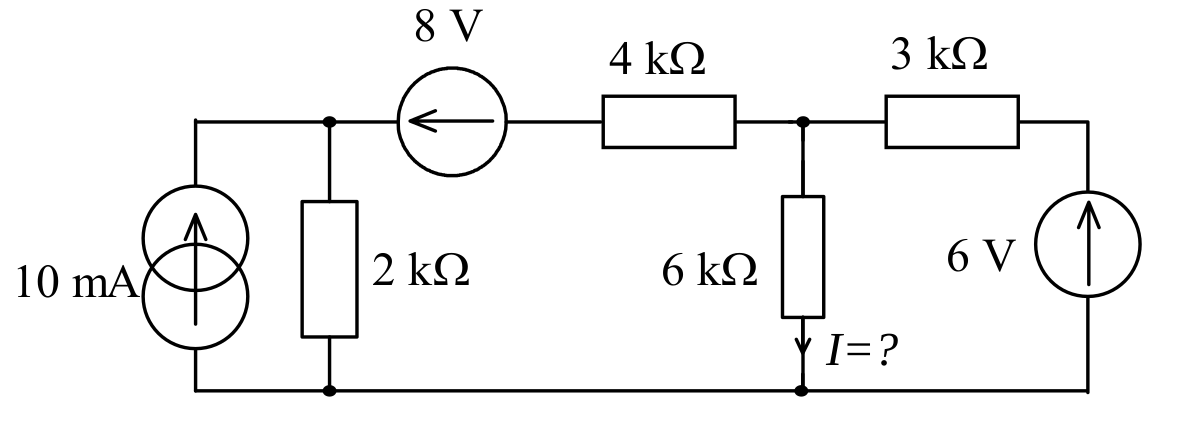
\includegraphics[width = 0.7\textwidth]{./images/Lista_1/Zadanie_5.png}
\end{figure}
\paragraph{Rozwiązanie}
\begin{flushleft}
  Pierwsze co to zaznaczmy co z czym połączymy.
\end{flushleft}
\begin{figure}[H]
  \centering
  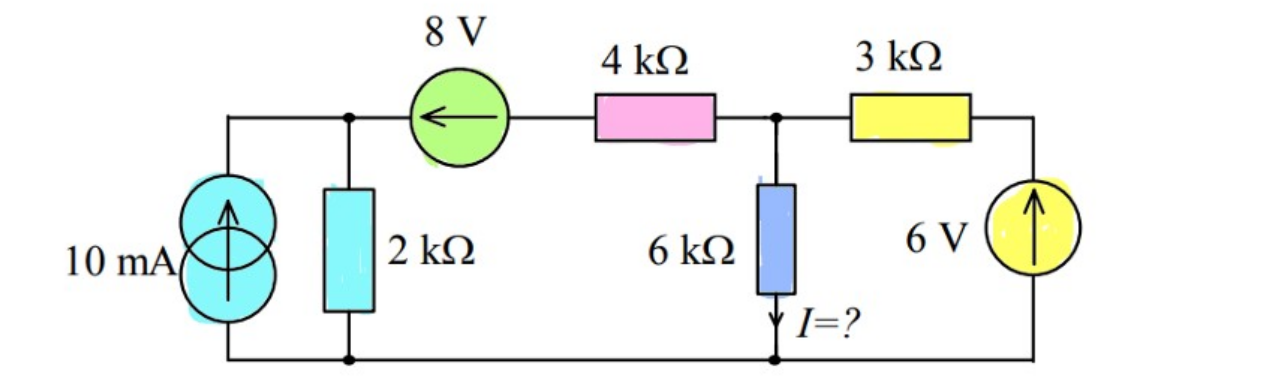
\includegraphics[width = 0.7\textwidth]{./images/Lista_1/Zadanie5_1.png}
\end{figure}

Pierwszą zamianą będzie zamiana rzeczywistego źródła prądowego na rzeczywiste
źródło napięciowe.
\begin{figure}[H]
  \centering
  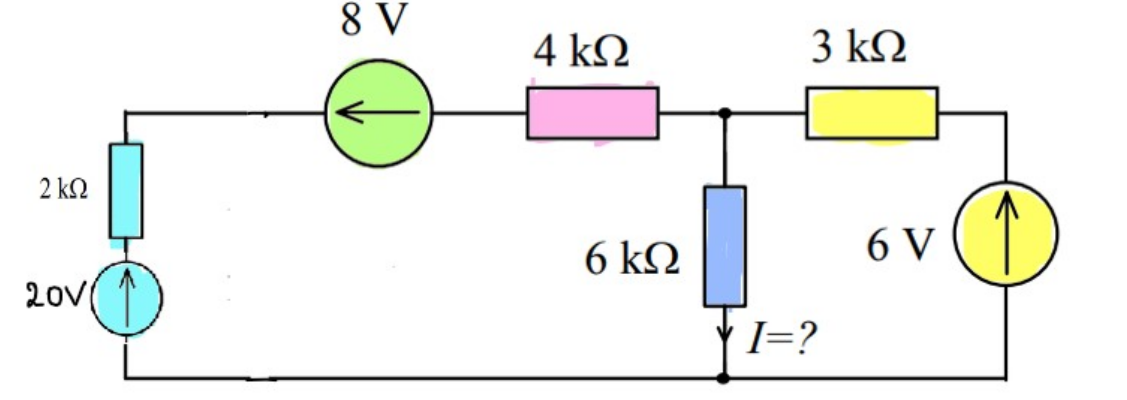
\includegraphics[width = 0.7\textwidth]{./images/Lista_1/Zadanie5_2.png}
\end{figure}

Połączmy teraz dwa rzeczywiste źródła napięciowe i dwa rezystory, które są
połączone szeregowo.
\begin{figure}[H]
  \centering
  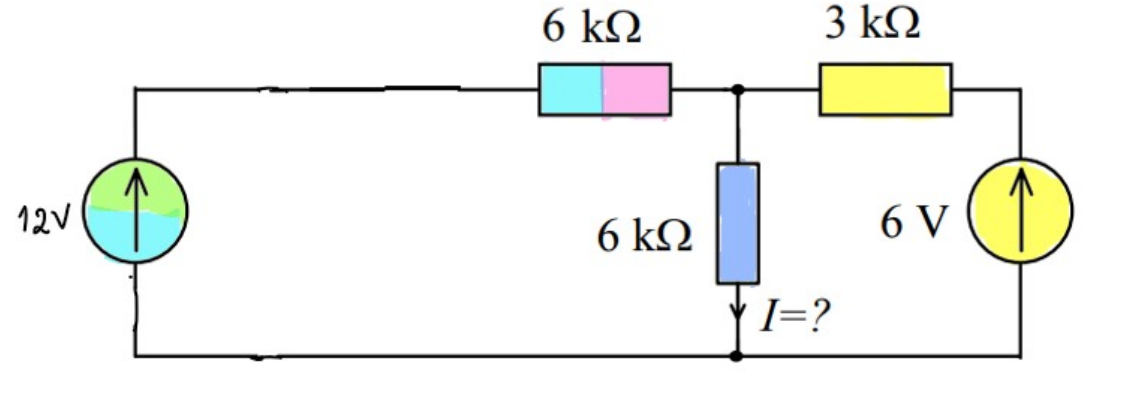
\includegraphics[width = 0.7\textwidth]{./images/Lista_1/Zadanie5_3.png}
\end{figure}
$$
  \Downarrow
$$
\begin{figure}[H]
  \centering
  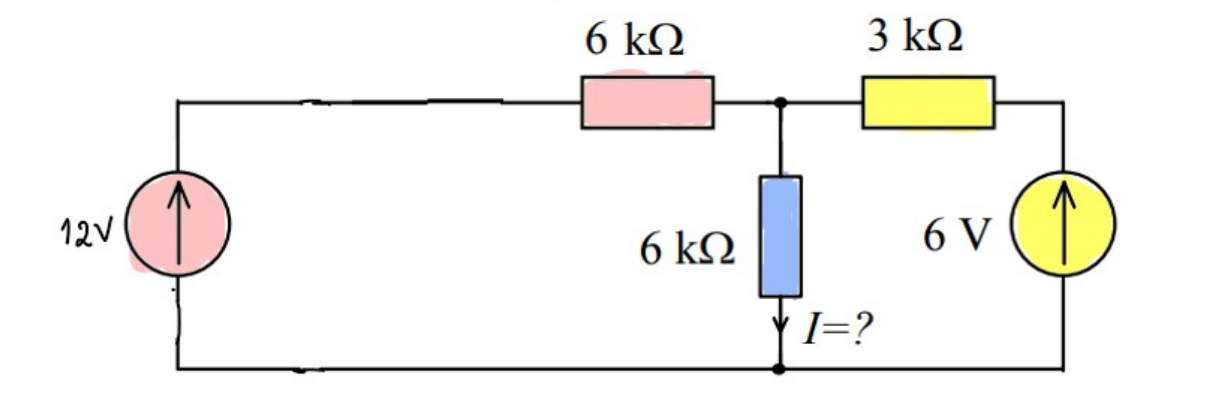
\includegraphics[width = 0.7\textwidth]{./images/Lista_1/Zadanie5_4.png}
\end{figure}

Zamieńmy teraz oba rzeczywiste źródła napięcia na rzeczywiste źródła prądowe.
\begin{figure}[H]
  \centering
  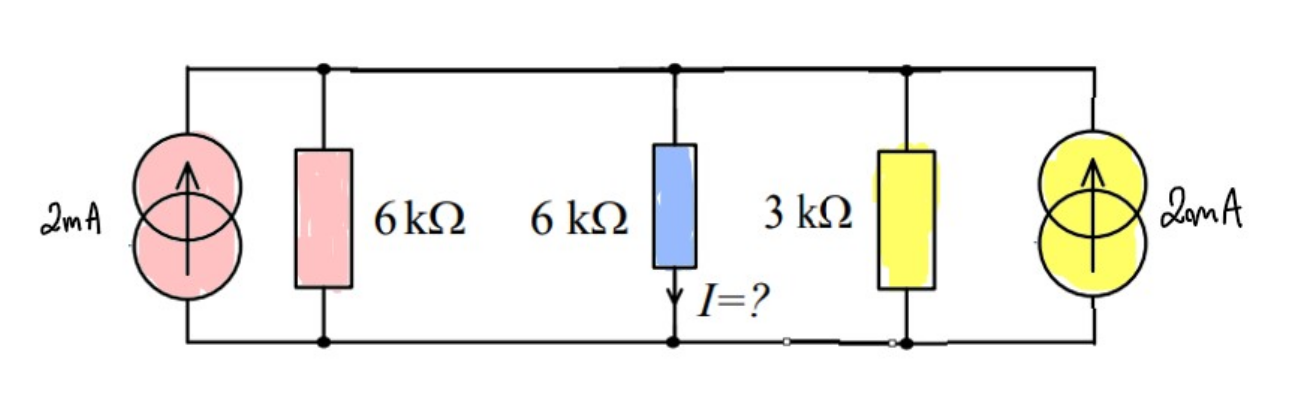
\includegraphics[width = 0.7\textwidth]{./images/Lista_1/Zadanie5_5.png}
\end{figure}

Na koniec wystarczy połączyć dwa źródła prądowe w jedno.
\begin{figure}[H]
  \centering
  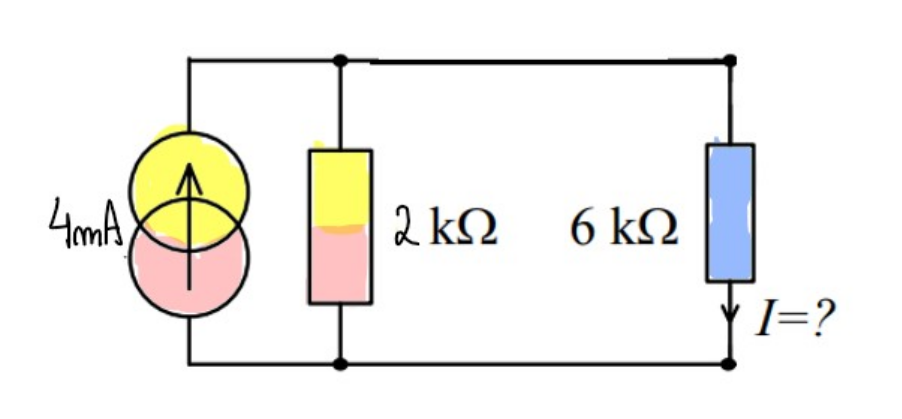
\includegraphics[width = 0.5\textwidth]{./images/Lista_1/Zadanie5_6.png}
\end{figure}

Na koniec z dzielnika prądowego możemy policzyć prąd $I$.
$$
  I = 4 \cdot \frac{2}{2+6} = 1\; mA
$$

% Zadanie 6
\subsection{Zadanie 6}
\textbf{Wypisać kompletny układ równań niezależnych opisujących obwody przedstawione na
  rys.}
\begin{figure}[H]
  \centering
  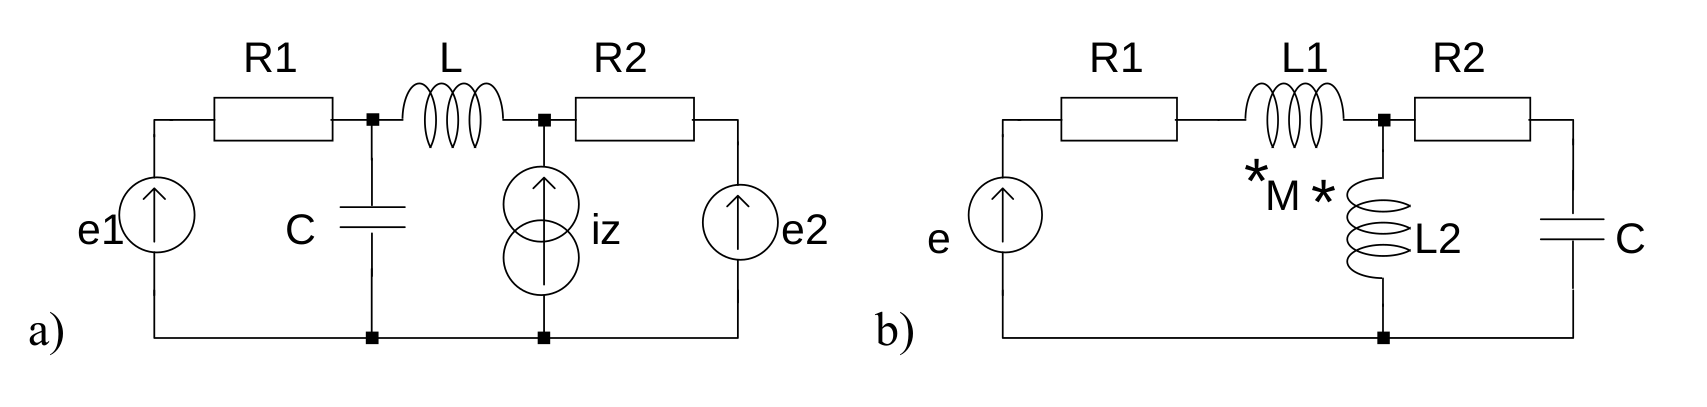
\includegraphics[width = \textwidth]{./images/Lista_1/Zadanie_6.png}
\end{figure}

%---------------------------- LISTA 2 -----------------------------------------
\section{Lista 2}
% Zadanie 1
\subsection{Zadanie 1}
\textbf{Znaleźć zespolone wartości skuteczne następujących prądów i napięć:}
\begin{enumerate}[label=\alph*)]
  \item $u(t) = 12\sqrt{2} \sin\left( 150t-\dfrac{7}{12}\pi \right)$,
  \item $i(t) = 5\sqrt{2}\cos\left( 35t+\dfrac{3}{4}\pi \right)$,
  \item $u(t) = 10\sin\left(100t+\dfrac{2}{3}\pi\right)+
          20\cos\left(100t-\dfrac{\pi}{2}\right)$,
  \item $u(t) = 5\sin\left(200t+75^\circ\right)-4\cos\left(200t-75^\circ\right)$.
\end{enumerate}

\paragraph{Rozwiązanie}
\begin{enumerate}[label=\alph*)]
  \item Zacznijmy od wyznaczenia wartości skutecznej napięcia
        $$
          u_{sk} = \frac{12\sqrt{2}}{\sqrt{2}} = 12.
        $$
        Zapiszmy teraz to w postaci wykładniczej
        $$
          \underline{U} = 12e^{-j\frac{7}{12}\pi} = 12e^{-j105^\circ}.
        $$
  \item Pierwszą rzeczą będzie zamienienie $\cos$ na $\sin$
        $$
          i(t) = 5\sqrt{2}\sin\left(35t+\frac{3}{4}\pi+\frac{\pi}{2}\right).
        $$
        Policzmy teraz wartość skuteczną
        $$
          i_{sk} = \frac{5\sqrt{2}}{\sqrt{2}} = 5.
        $$
        Na koniec wystarczy zapisać to w postaci wykładniczej
        $$
          \underline{I} = 5e^{j\left(\frac{3}{4}\pi+\frac{\pi}{2}\right)} =
          5e^{-j\frac{3}{4}\pi}.
        $$
  \item Pierwszą rzeczą będzie przekształcenie sumy sinusoidy i cosinusoidy na
        sumę dwóch składników wykładniczych. Możemy od razu też wyciągnąć wartość
        $\omega_0$.
        $$
          \underline{U} = \dfrac{10}{\sqrt{2}}e^{j\frac{2}{3}\pi} +
          \dfrac{20}{\sqrt{2}}e^{j\left(-\frac{1}{2}\pi+\frac{1}{2}\pi\right)}, \quad
          \omega_0 = 100\; \frac{rad}{s}
        $$

        Przekształćmy to teraz do prostszej postaci oraz zamieńmy kąt na taki z
        zakresu do $\dfrac{\pi}{2}$.
        $$
          \underline{U} = 5\sqrt{2}\left(2+e^{j\left(\pi-\frac{1}{3}\pi\right)}\right)
        $$
        $$
          \underline{U} = 5\sqrt{2}\left(2-e^{-j\frac{1}{3}\pi}\right)
        $$

        Następnym krokiem będzie zamiana postaci wykładniczej na postać
        algebraiczną.
        $$
          \underline{U} = 5\sqrt{2}\left(2-\cos\left(-\dfrac{1}{3}\pi\right)
          -j\sin\left(-\dfrac{1}{3}\pi\right)\right)
        $$

        $$
          \underline{U} = 5\sqrt{2}\left(2-\dfrac{1}{2}+j\dfrac{\sqrt{3}}{2}\right)
        $$
        $$
          \underline{U} = 5\sqrt{2}\left(\dfrac{3}{2}+j\dfrac{\sqrt{3}}{2}\right)
        $$
        \begin{equation}\label{2.1c_algebraiczna}
          \underline{U} = \dfrac{5}{2}\sqrt{2}\left(3+j\sqrt{3}\right)
        \end{equation}

        Postać algebraiczna jak w równaniu \ref{2.1c_algebraiczna} pozwoli zamienić
        to równanie na jeden wskaz wykładniczy.
        $$
          \underline{U} = \dfrac{5}{2}\sqrt{2}\sqrt{9+3}\cdot e^{j\arctan\left(
              \frac{\sqrt{3}}{3}\right)}
        $$
        $$
          \underline{U} = 5\sqrt{2}\sqrt{3}\cdot e^{j\frac{\pi}{6}}
        $$
        \begin{equation}\label{2.1c_wykladnicza}
          \underline{U} = 5\sqrt{6}\cdot e^{j\frac{\pi}{6}}
        \end{equation}

        Korzystając z równania \ref{2.1c_wykladnicza} w postaci wykładniczej
        możemy zapisać to jako jeden przebieg sinusoidalny.
        $$
          u(t) = 5\sqrt{6}\sqrt{2}\cdot\sin\left(\omega_0 t+\dfrac{\pi}{6}\right)
        $$
        $$
          u(t) = 10\sqrt{3}\cdot\sin\left(100 t+\dfrac{\pi}{6}\right)\: V
        $$
  \item Tak jak w poprzednim podpunkcie zapiszmy to w postaci dwóch wskazów
        wykładniczych, oraz wypiszmy wartość $\omega_0$.
        $$
          \underline{U} = \frac{5}{\sqrt{2}}\cdot e^{j75^\circ}-\frac{4}{\sqrt{2}}
          \cdot e^{j(-75^\circ+90^\circ)}, \quad \omega_0 = 200\; \frac{rad}{s}
        $$

        Przekształcając dalej otrzymamy postać jak w równaniu \ref{2.1d_wykladnicza}.
        $$
          \underline{U} = \frac{1}{\sqrt{2}}\left(5e^{j(45^\circ+30^\circ)}
          -4e^{j(90^\circ-45^\circ-30^\circ)} \right)
        $$
        $$
          \underline{U} = \frac{1}{\sqrt{2}}\left(5e^{j(45^\circ+30^\circ)}
          -4e^{j(45^\circ-30^\circ)} \right)
        $$
        \begin{equation}\label{2.1d_wykladnicza}
          \underline{U} = \frac{e^{j45^\circ}}{\sqrt{2}}
          \left(5e^{j30^\circ}-4e^{-j30^\circ} \right)
        \end{equation}

        Suma dwóch elementów wykładniczych pozwoli nam zapisać to w postaci
        algebraicznej.
        $$
          \underline{U} = \frac{1}{\sqrt{2}}\frac{1}{\sqrt{2}}(1+j)
          \left(5\frac{\sqrt{3}}{2}+j\frac{5}{2}-4\frac{\sqrt{3}}{2}+j\frac{4}{2}\right)
        $$
        $$
          \underline{U} = \frac{1}{4}(1+j)\left(\sqrt{3}+j9\right)
        $$
        \begin{equation}\label{2.1d_algebraiczna}
          \underline{U} = -\frac{1}{4}\left(9-\sqrt{3}-j\left(9+\sqrt{3}\right)\right)
        \end{equation}

        Korzystając z równania \ref{2.1d_algebraiczna} zapisujemy to w postaci
        jednej eksponenty jak w równaniu \ref{2.1d_wykladnicza2}.
        $$
          \underline{U} = \frac{1}{4}\sqrt{1+1}\sqrt{3+81} \cdot
          e^{45^\circ+\arctan\left(\frac{9}{\sqrt{3}}\right)}
        $$
        \begin{equation}\label{2.1d_wykladnicza2}
          \underline{U} = \frac{1}{2}\sqrt{2}\sqrt{21}\cdot
          e^{45^\circ+\arctan\left(3\sqrt{3}\right)}
        \end{equation}

        Na koniec wystarczy to wszystko zapisac w postaci przebiegu sinusoidalnego.
        $$
          u(t) = \frac{1}{2}\sqrt{2}\sqrt{21}\sqrt{2}\cdot
          \sin\left(\omega_0 t+45^\circ+\arctan\left(3\sqrt{3}\right)\right)
        $$
        $$
          u(t) = \sqrt{21}\cdot
          \sin\left(200t+45^\circ+\arctan\left(3\sqrt{3}\right)\right)\: V
        $$
        $$
          u(t) \approx 4,583 \sin\left(200t+124,11^\circ\right) =
          4,583 \cos\left(200t+34,11^\circ\right)\: V
        $$
\end{enumerate}

% Zadanie 2
\subsection{Zadanie 2}
\textbf{Przedstawić jako funkcje czasu następujące prądy i napięcia:}
\begin{enumerate}[label=\alph*)]
  \item $\underline{U}_1 = -1-j, \; \omega = 120\textrm{ rad/s}$,
  \item $\underline{I}_2 = 10j, \; \omega = 300\textrm{ rad/s}$,
  \item $\underline{U}_3 = 8e^{-j\frac{2\pi}{3}}+4e^{\frac{\pi}{3}},\;
          \omega = 240\textrm{ rad/s}$,
  \item $\underline{I}_4 = -2+j4, \; \omega = \pi$.
\end{enumerate}

\paragraph{Rozwiązanie}
\begin{enumerate}[label=\alph*)]
  \item Zacznijmy od wyliczenia modułu i wartości kąta
        $$
          |z| = \sqrt{(-1)^2+(-1)^2} = \sqrt{2},
        $$
        $$
          \left\{
          \begin{array}{rl}
            \cos(\phi) = & \dfrac{-1}{\sqrt{2}} \\
            \sin(\phi) = & \dfrac{-1}{\sqrt{2}}
          \end{array}
          \right.
          \quad \Rightarrow \quad \phi = 225^\circ.
        $$
        Korzystając z tych wartości możemy zapisać $u_1(t)$ w postaci
        wykładniczej
        \begin{equation}\label{2.1a_wykladnicza}
          u_1(t) = \sqrt{2}e^{j225^\circ} = \sqrt{2}e^{-j135^\circ}.
        \end{equation}
        Następnie korzystając z równania \ref{2.1a_wykladnicza} zapisujemy
        przebieg sinusoidalny
        $$
          u_1(t) = \sqrt{2}\cdot\sqrt{2}\sin\left(120t-\frac{3}{4}\pi\right).
        $$
  \item Zacznijmy od wyliczenia modułu i wartości kąta
        $$
          |z| = \sqrt{0^2+10^2} = 10,
        $$
        $$
          \left\{
          \begin{array}{rl}
            \cos(\phi) = & \frac{0}{10}  \\
            \sin(\phi) = & \frac{10}{10}
          \end{array}
          \right.
          \quad \Rightarrow \quad \phi = 90^\circ.
        $$
        Korzystając z tych wartości możemy zapisać $u_2(t)$ w postaci
        wykładniczej
        \begin{equation}\label{2.1b_wykladnicza}
          u_1(t) = 10e^{j90^\circ}.
        \end{equation}
        Następnie korzystając z równania \ref{2.1b_wykladnicza} zapisujemy
        przebieg sinusoidalny
        $$
          u_1(t) = 10\cdot\sqrt{2}\sin\left(300t+\frac{\pi}{2}\right).
        $$
  \item Na początek zapiszmy nasze równanie jako jeden wskaz zespolony.
        $$
          \underline{U} = 8e^{j\left(-\pi+\frac{1}{3}\pi\right)}
          +4e^{j\frac{1}{3}\pi}
        $$
        $$
          \underline{U} = -8e^{j\frac{1}{3}\pi}+4e^{j\frac{1}{3}\pi}
        $$
        \begin{equation}\label{2.2c_wykladnicza}
          \underline{U} = -4e^{j\frac{1}{3}\pi}
        \end{equation}

        Korzystając z równania \ref{2.2c_wykladnicza}, możemy zapisać przebieg
        sinusoidalny.
        $$
          u(t) = -4\sqrt{2}\cdot\sin\left(240t+\frac{\pi}{3}\right)
        $$
  \item Przekształćmy postać algebraiczną do prostszej postaci
        $$
          \underline{I} = -2+j4 = -2(1-j2),
        $$
        a następnie zapiszmy to w postaci wykładniczej
        \begin{equation}\label{2.2d_wykladnicza}
          \underline{I} = -2\sqrt{1+4}\cdot e^{-j\arctan(2)} =
          -2\sqrt{5}\cdot e^{-j\arctan(2)}.
        \end{equation}

        Na koniec możemy zapisać to w przebiegu sinusoidalnym korzystając z
        równania \ref{2.2d_wykladnicza}.
        $$
          i(t) = -2\sqrt{5}\sqrt{2}\cdot \sin\left(\pi t-\arctan(2)\right)
        $$
        $$
          i(t) \approx -6,325\sin\left(\pi t-63,43^\circ\right) =
          6,325\sin\left(\pi t-116,57^\circ\right)\: A
        $$
\end{enumerate}

% Zadanie 3
\subsection{Zadanie 3}
\textbf{Wyznaczyć amplitudę i fazę początkową napięcia $u(t)$, gdzie}
$$
  u(t) = 35\sin(\omega t)+45\cos(\omega t).
$$

Pierwsze co musimy zrobić to zamienić $\cos$ na $\sin$.
\begin{equation}\label{2.3_sincos}
  u(t) = 35\sin(\omega t)+45\sin(\omega t+\frac{\pi}{2})
\end{equation}
Przedstawmy teraz równanie \ref{2.3_sincos} w postaci wskazów zespolonych
$$
  u(t) = \frac{35}{\sqrt{2}}e^{0}+\frac{55}{\sqrt{2}}e^{j\frac{\pi}{2}},
$$
a następnie przekształcamy je do postaci algebraicznej
\begin{equation}\label{2.3_algebraiczna}
  u(t) = \frac{1}{\sqrt{2}}\left(35e^0+45e^{j\frac{\pi}{2}}\right) =
  \frac{1}{\sqrt{2}}\left(35+j45\right).
\end{equation}

Aby przedstawić równanie \ref{2.3_algebraiczna} w postaci wykładniczej musimy
policzyć moduł oraz wartość kąta.
$$
  |z| = \sqrt{35^2+45^2} = 5\sqrt{130}
$$
$$
  \left\{
  \begin{array}{rl}
    \cos(\phi) = & \dfrac{35}{5\sqrt{130}} \\
    \sin(\phi) = & \dfrac{45}{5\sqrt{130}}
  \end{array}
  \right.
  \quad \Rightarrow \quad \phi = 52,13^\circ
$$
Teraz możemy przedstawić równanie \ref{2.3_algebraiczna} w postaci wykładniczej
\begin{equation}\label{2.3_wykładnicza}
  u(t) = 5\sqrt{65}e^{j52,13^\circ}.
\end{equation}

Korzystając z równania \ref{2.3_wykładnicza} możemy to zapisać w postaci
sinusoidy
$$
  u(t) = 5\sqrt{130}\sin\left(\omega t+ 52,13^\circ\right),
$$
gdzie $5\sqrt{130}$ to \textbf{amplituda}, a $52,13^\circ$ to \textbf{faza
  początkowa}.

% Zadanie 4
\subsection{Zadanie 4}
\textbf{Wyznaczyć napięcie na kondensatorze $u_c(t)$.}\\
\begin{minipage}{0.4\textwidth}
  \begin{figure}[H]
    \centering
    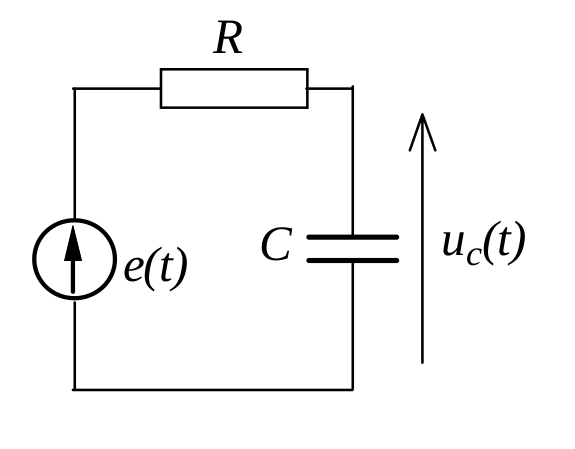
\includegraphics[width = \textwidth]{./images/Lista_2/Zadanie_4.png}
  \end{figure}
\end{minipage}
\hspace*{0.5cm}
\begin{minipage}{0.4\textwidth}
  $$
    e(t) = 10\sin\left(10^3+\dfrac{5}{9}\pi\right)\: V,
  $$
  $$
    C = 10 \mu F,
  $$
  $$
    R = 50 \Omega.
  $$
\end{minipage}

Zapiszmy na początek wartość źródła w postaci wykładniczej.
$$
  \underline{E}=\frac{10}{\sqrt{2}}e^{j\frac{5}{9}\pi}, \quad
  \omega_0 = 10^3\; \frac{rad}{s}
$$
\begin{equation}\label{2.4_impedancja}
  \underline{Z}_c = \frac{1}{j\omega_0 C}
\end{equation}
Z dzielnika napięciowego wyznaczamy napięcie na kondensatorze.
\begin{equation}\label{2.4_napiecieDzielnik}
  \underline{U}_c = \underline{E}\frac{\underline{Z}_c}{R+\underline{Z}_c}
\end{equation}

Wstawiając wzór \ref{2.4_impedancja} do równania \ref{2.4_napiecieDzielnik}
otrzymujemy wzór końcowy na napięcie zespolone.
\begin{equation}\label{2.4_napiecieWzor}
  \underline{U}_c = \frac{\underline{E}}{1+j\omega_0 RC}
\end{equation}
Wstawiając odpowiednie wartości do równania \ref{2.4_napiecieWzor}, a następnie
przekształcając je do prostszej postaci otrzymujemy równanie \ref{2.4_wykladnicza}.
$$
  \underline{U}_c = \frac{10}{\sqrt{2}}e^{j\frac{5}{9}\pi} \cdot
  \frac{1}{1+j\frac{1}{2}}
$$
$$
  \underline{U}_c = \frac{20}{\sqrt{2}(2+j)}e^{j\frac{5}{9}\pi}
$$
\begin{equation}\label{2.4_wykladnicza}
  \underline{U}_c = \frac{20}{\sqrt{2}\sqrt{5}}e^{j\left(\frac{5}{9}\pi-\arctan
  \left(\frac{1}{2}\right)\right)} =
  2\sqrt{10}\cdot e^{j\left(\frac{5}{9}\pi-\arctan\left(\frac{1}{2}\right)\right)}
\end{equation}

Korzystając z postaci wykładniczej w równaniu \ref{2.4_wykladnicza} zapisujemy
napięcie na kondensatorze w postaci sinusoidalnej.
$$
  u_c(t) = 2\sqrt{10}\sqrt{2}\cdot\sin\left(\omega_0t+\frac{5}{9}\pi-
  \arctan\left(\frac{1}{2}\right)\right)
$$
$$
  u_c(t) = 4\sqrt{5}\cdot\sin\left(\omega_0t+\frac{5}{9}\pi-
  \arctan\left(\frac{1}{2}\right)\right)
$$
$$
  u_c(t) \approx 8,944\sin\left(10^3t+73,43\right)\: V
$$

% Zadanie 5
\subsection{Zadanie 5}
\textbf{Wyznaczyć wartość rezystancji $R_2$, którą należy dołączyć do zacisków
  1 1’, aby $\left|\dfrac{\underline{U}}{\underline{E}}\right| = k$.\\
  Do obliczeń przyjąć następujące dane: $R_1 = 100\Omega$, $\frac{1}{\omega C} =
    50\Omega$, $k=0,2$.}
\begin{figure}[H]
  \centering
  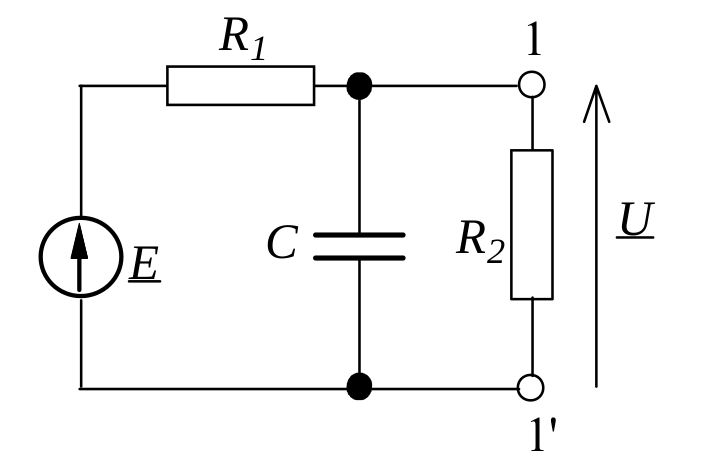
\includegraphics[width = 0.4\textwidth]{./images/Lista_2/Zadanie_5.png}
\end{figure}

Najpierw powinniśmy wyznaczyć stosunek podziału napięcia w dzielniku
napięciowym.
\begin{equation}\label{2.5_dzielnik}
  \underline{k} = \frac{\underline{U}}{\underline{E}} = \frac{\underline{Z}}
  {R_1+\underline{Z}}
\end{equation}

\begin{equation}\label{2.5_impedancja}
  \underline{Z} = \frac{1}{\dfrac{1}{R_2}+j\omega_0C} =
  \frac{R_2}{1+j\omega_0R_2C}
\end{equation}

Wstawiając do równania \ref{2.5_dzielnik} wyprowadzone wartości w równaniu
\ref{2.5_impedancja} otrzymujemy wzór końcowy na stosunek napięć
$$
  \underline{k} = \frac{R_2}{R_2+R_1(1+j\omega_0R_2C)} =
  \frac{1}{1+\dfrac{R_1}{R_2}+j\omega_0R_1C}.
$$

Ze względu, że w danych zadania mamy podany moduł zespolonego $k$, a kwadraty
modułów są równe możemy wyprowadzić następujące równanie
$$
  k^2=|\underline{k}|^2=\frac{1}{\left(1+\dfrac{R_1}{R_2}\right)^2+
    \left(\omega_0R_1C\right)^2}.
$$
Przekształcając dalej to równanie otrzymujemy wzór na $R_2$, co przedstawia
równanie \ref{2.5_rezystancja}.
$$
  \frac{1}{k^2} = \left(1+\dfrac{R_1}{R_2}\right)^2+\left(\omega_0R_1C\right)^2
$$
$$
  1+\frac{R_1}{R_2} = \sqrt{\frac{1}{k^2}-\left(\omega_0R_1C\right)^2}
$$

\begin{equation}\label{2.5_rezystancja}
  R_2 = \frac{R_1}{\sqrt{\frac{1}{k^2}-\left(\omega_0R_1C\right)^2}-1}
\end{equation}

Podstawiając odpowiedni wartośći do równania \ref{2.5_rezystancja} obliczamy
końcowy wynik.
$$
  R_2 = \frac{100}{\sqrt{\frac{1}{0,2^2}-4}-1} = \frac{100}{\sqrt{21}-1}
  \approx 27,91\: \Omega
$$

% Zadanie 6
\subsection{Zadanie 6}
\textbf{W obwodzie pokazanym na rysunku panuje stan ustalony. Obliczyć napięcie
  $u(t)$ posługując się metodą symboliczną.}\\
\begin{minipage}{0.6\textwidth}
  \begin{figure}[H]
    \centering
    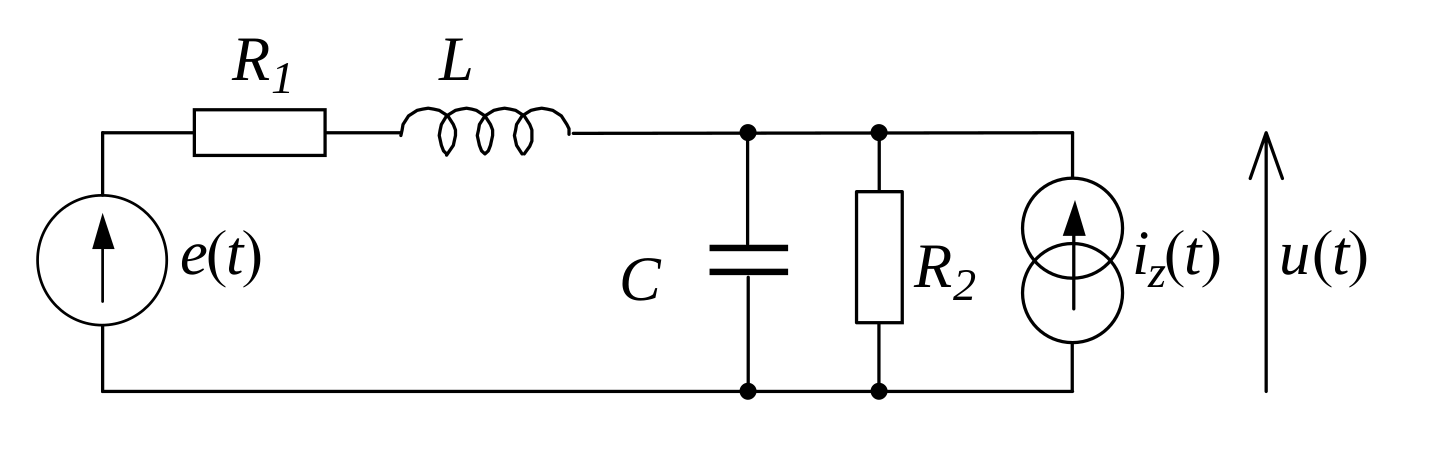
\includegraphics[width = \textwidth]{./images/Lista_2/Zadanie_6.png}
  \end{figure}
\end{minipage}
\hspace*{0.4cm}
\begin{minipage}{0.35\textwidth}
  $$
    e(t) = 10\sin\left(\omega t\right)\: V,
  $$
  $$
    i_z(t) = 0,05\sin\left(\omega t+30^\circ\right)\: A,
  $$
  $$
    R_1 = 100\; \Omega, \: R_2 = 200\; \Omega,
  $$
  $$
    L = 10,61\; mH,\: C = 0,2653\; \mu F,
  $$
  $$
    f = 3\;  kHz.
  $$
\end{minipage}\\[0.3cm]
\vspace*{0.3cm}

Pierwsze co powinniśmy zrobić rozwiązując zadania z metody symbolicznej to
przedstawić wartości sinusoidalne poprzez odpowiednie wskazy zespolone.
$$
  \underline{E} = \frac{10}{\sqrt{2}} = 5\sqrt{2}\: V
$$
$$
  \underline{I}_z = \frac{0,05}{\sqrt{2}}e^{j30^\circ} =0,0124\sqrt{2}(\sqrt{3}+j)\: A
$$
$$
  \omega_0 = 2\pi f_0 \approx 18850\; \frac{rad}{s}
$$

Następnym krokiem powinno być obliczenie impedancji $Z_1$. Jest to impedancja
szeregowo połączonego rezystora $R_1$ oraz induktora $L$.
\begin{equation}\label{2.6_impedancja_Z_1}
  \underline{Z}_1 = R_1+j\omega_0L
\end{equation}
Wstawiając odpowiednie wartości do równania \ref{2.6_impedancja_Z_1} otrzymujemy
wartość tej impedancji.
$$
  \underline{Z}_1 \approx 100 + j18850\cdot10,61\cdot10^{-3} = 100+j200\; \Omega
$$

W kolejnym kroku należy obliczyć impedancję na dwójniku złożonym z kondensatora
i rezystora $R_2$. Impedancja ta jest odwrotnością sumy admitancji tych dwóch
gałęzi co przedstawia wzór \ref{2.6_impedancja_Z_2}.
\begin{equation}\label{2.6_impedancja_Z_2}
  \underline{Z}_2 = \frac{1}{\frac{1}{R_2}+j\omega_0C} = \frac{R_2}{1+j\omega_0R_2C}
\end{equation}
Podstawiając odpowiednie wartości do równania \ref{2.6_impedancja_Z_2}
otrzymujemy wartość impedancji $Z_2$.
$$
  \underline{Z}_2 \approx \frac{200}{1+j18850\cdot200\cdot0,2653\cdot10^{-6}} =
  99,98-j100\; \Omega
$$

Następnie zastępujemy rzeczywiste źródło napięcia, rzeczywistym źródłem prądowym.
Wartość końcowa będzie sumą wartości dwóch źródeł prądowych, które będą
połączone równolegle.
$$
  \underline{I}_{za} = \underline{I}_z + \frac{\underline{E}}{\underline{Z}_1}
$$
$$
  \underline{I}_{za} \approx 0,0125\sqrt{2}\left(\sqrt{3}+j\right) +
  \frac{5\sqrt{2}}{100+j200} \approx 0,0448-j0,0110\; A
$$

Ze względu, że obie impedancje połączone są równolegle, można je zastąpić jedną
impedancją zastępczą, co pokazuje równanie \ref{2.6_impedancja_zastepcza}.
\begin{equation}\label{2.6_impedancja_zastepcza}
  \underline{Z} = \frac{\underline{Z}_1\underline{Z}_2}{\underline{Z}_1+\underline{Z}_2}
\end{equation}
Wyliczmy teraz tą impedancję wstawiając odpowienie wartości do równania
\ref{2.6_impedancja_zastepcza}.
$$
  \underline{Z} \approx 140 - j20\; \Omega
$$

Zgodnie z prawem Ohma spadek napięcia na źródle $\underline{I}_{za}$ będzie
przedstawiony równaniem \ref{2.6_spadek_napiecia}.
\begin{equation}\label{2.6_spadek_napiecia}
  \underline{U} = \underline{Z}\cdot\underline{I}_{za}
\end{equation}
Obliczamy teraz wartość tego napięcia i przedstawiamy w postaci algebraicznej
oraz wykładniczej.
$$
  \underline{U} \approx (140 - j20)\cdot(0,0448-j0,0110) \approx 6,054+j2,381
  \approx 6,51e^{-j21,47^\circ}
$$

Na koniec wystarczy odtworzyć to w postaci sinusoidy.
$$
  u(t) \approx 6,51\sqrt{2}\cdot\sin(\omega_0t-21,47) \approx
  9,20\sin(\omega_0t-21,47)\; V
$$

\section{Lista 3}
\subsection{Zadanie 1}
\textbf{Obliczyć napięcie $u(t)$ w stanie ustalonym.}
\begin{figure}[H]
  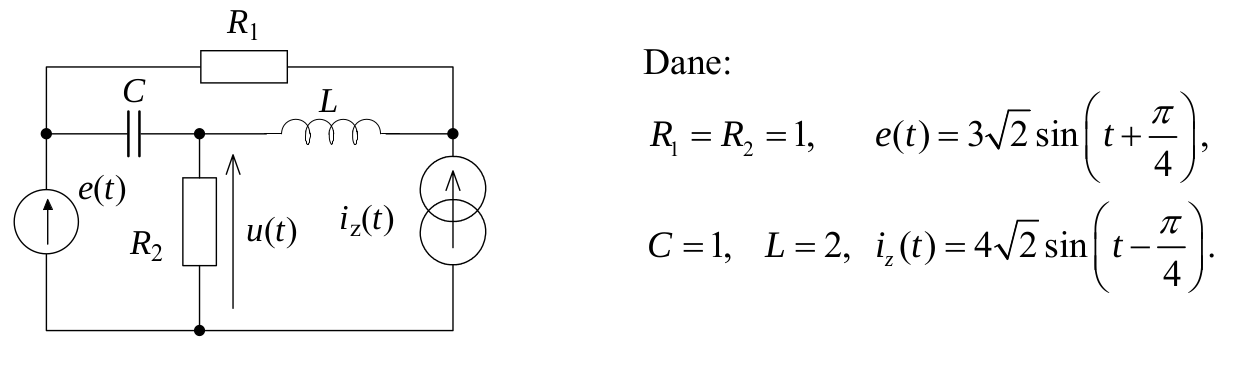
\includegraphics[width = 0.8\textwidth]{./images/Lista_3/Zadanie_1.png}
\end{figure}

Przekształćmy na początek postacie sinusoidalne na algebraiczne
\begin{equation*}
  e(t) = 3\sqrt{2}\sin\left(t+\frac{\pi}{4}\right) = 3e^{j45^\circ} =
  \frac{3\sqrt{2}}{2}+\frac{3\sqrt{2}}{2}j,
\end{equation*}
\begin{equation*}
  i_z(t) = 4\sqrt{2}\sin\left(t-\frac{\pi}{4}\right)= 4e^{-j45^\circ} =
  2\sqrt{2}-2\sqrt{2}j.
\end{equation*}

\begin{figure}[H]
  \centering
  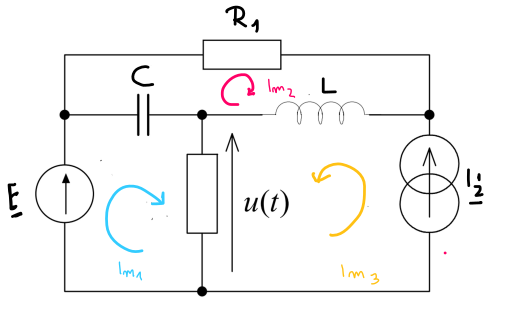
\includegraphics[width = 0.4\textwidth]{./images/Lista_3/3.1.png}
\end{figure}

Korzystając z \textbf{metody prądów oczkowych} możemy zapisać układ trzech równań, ponieważ
są trzy niezależne oczka.
\begin{equation}\label{3.1_uklad_rownan}
  \left\{
  \begin{array}{rl}
    \underline{E} =      & \underline{I}_{m1}\left(\frac{1}{j\omega C}+R_2\right) + \underline{I}_{m3}\cdot R_2-\underline{I}_{m2}\cdot \frac{1}{j\omega C}                 \\
    0 =                  & \underline{I}_{m2}\left(R_1+j\omega L+\frac{1}{j\omega C}\right)+\underline{I}_{m3}\cdot j\omega L - \underline{I}_{m1}\cdot \frac{1}{j\omega C} \\
    \underline{I}_{m3} = & \underline{I}_z
  \end{array}
  \right.
\end{equation}
Układ równań \ref{3.1_uklad_rownan} można zapisać w postaci macierzowej co znacznie
ułatwi wyliczanie wartości.
\begin{equation*}
  \begin{bmatrix}
    \frac{1}{j\omega C}+R_2 & -\frac{1}{j\omega C}              & R_2       \\
    -\frac{1}{j\omega C}    & R_1+j\omega L+\frac{1}{j\omega C} & j\omega L \\
    0                       & 0                                 & 1
  \end{bmatrix}
  \cdot
  \begin{bmatrix}
    \underline{I}_{m1} \\
    \underline{I}_{m2} \\
    \underline{I}_{m3}
  \end{bmatrix}
  =
  \begin{bmatrix}
    \underline{E} \\
    0             \\
    \underline{I}_z
  \end{bmatrix}
\end{equation*}
Wstawiając dalej wartości otrzymujemy równanie macierzowe \ref{3.1_macierzowe}
\begin{equation}\label{3.1_macierzowe}
  \begin{bmatrix}
    1-j & j   & 1  \\
    j   & 1+j & 2j \\
    0   & 0   & 1
  \end{bmatrix}
  \cdot
  \begin{bmatrix}
    \underline{I}_{m1} \\
    \underline{I}_{m2} \\
    \underline{I}_{m3}
  \end{bmatrix}
  =
  \begin{bmatrix}
    \underline{E} \\
    0             \\
    \underline{I}_z
  \end{bmatrix}.
\end{equation}

Wyznaczając $\underline{I}_{m3}$ i wstawiając do równań możemy układ równań
\ref{3.1_uklad_rownan} przekształcić do równania macierzowego \ref{3.1_macierzowe2}.
\begin{equation}\label{3.1_macierzowe2}
  \begin{bmatrix}
    1-j & j   \\
    j   & 1+j \\
  \end{bmatrix}
  \cdot
  \begin{bmatrix}
    \underline{I}_{m1} \\
    \underline{I}_{m2} \\
  \end{bmatrix}
  =
  \begin{bmatrix}
    \underline{E} - \underline{I}_z \\
    -2j \cdot \underline{I}_z
  \end{bmatrix}.
\end{equation}
Wyliczmy teraz przeliczone na samym początku wartości i wstawmy do równania
\ref{3.1_macierzowe2}.
\begin{equation*}
  \underline{E} - \underline{I}_z = 3e^{j45^\circ} - 4e^{-j45^\circ} =
  -\frac{\sqrt{2}}{2}+\frac{7\sqrt{2}}{2}j
\end{equation*}
\begin{equation*}
  - \underline{I}_z \cdot 2j = (2\sqrt{2}-2\sqrt{2}j)\cdot 2j =
  -4\sqrt{2}-4\sqrt{2}j
\end{equation*}

\begin{equation}\label{3.1_cramer}
  \begin{bmatrix}
    1-j & j   \\
    j   & 1+j \\
  \end{bmatrix}
  \cdot
  \begin{bmatrix}
    \underline{I}_{m1} \\
    \underline{I}_{m2} \\
  \end{bmatrix}
  =
  \begin{bmatrix}
    -\frac{\sqrt{2}}{2}+\frac{7\sqrt{2}}{2}j \\
    -4\sqrt{2}-4\sqrt{2}j
  \end{bmatrix}
\end{equation}

Równanie \ref{3.1_cramer} pozwoli nam teraz na wyliczenie wartości przy użyciu metody Cramera.
\begin{equation*}
  det\Delta
  \begin{bmatrix}
    1-j & j   \\
    j   & 1+j \\
  \end{bmatrix}
  = 3
\end{equation*}

\begin{equation*}
  det\; \underline{I}_{m1}
  \begin{bmatrix}
    -\frac{\sqrt{2}}{2}+\frac{7\sqrt{2}}{2}j & j   \\
    -4\sqrt{2}-4\sqrt{2}j                    & 1+j \\
  \end{bmatrix}
  = -8\sqrt{2} + 7\sqrt{2}j
  \quad \Rightarrow \quad
  \underline{I}_{m1} = \frac{det\; \underline{I}_{m1}}{det\Delta} =
  -\frac{8\sqrt{2}}{3}+\frac{7\sqrt{2}}{3}j
\end{equation*}

\begin{equation*}
  det\; \underline{I}_{m2}
  \begin{bmatrix}
    1-j & -\frac{\sqrt{2}}{2}+\frac{7\sqrt{2}}{2}j \\
    j   & -4\sqrt{2}-4\sqrt{2}j                    \\
  \end{bmatrix}
  = -\frac{9\sqrt{2}}{2}+\frac{\sqrt{2}}{2}j
  \quad \Rightarrow \quad
  \underline{I}_{m2} = \frac{det\; \underline{I}_{m2}}{det\Delta}
  = -\frac{9\sqrt{2}}{6}+\frac{\sqrt{2}}{6}j
\end{equation*}


Zgodnie z tym co zostało napisane na początku
\begin{equation*}
  u(t) = \left(\underline{I}_{m1}+\underline{I}_{m3}\right)\cdot R_2,
\end{equation*}
gdzie $\underline{I}_{m3} = \underline{I}_z$, możemy zapisać równanie na napięcie $u(t)$
w stanie ustalonym
\begin{equation}\label{3.1_napiecie}
  u(t) = \left(\underline{I}_{m1}+\underline{I}_z\right)\cdot R_2, \quad R_2 = 1\Omega.
\end{equation}
Wstawiając teraz odpowiednie wartości do równania \ref{3.1_napiecie} możemy zapisać
to napięcie w postaci algebraicznej
\begin{equation*}
  u(t) = -\frac{8\sqrt{2}}{3}+\frac{7\sqrt{2}}{3}j + 2\sqrt{2}-2\sqrt{2}j =
  -\frac{2\sqrt{2}}{3}+\frac{\sqrt{2}}{3}j,
\end{equation*}
a następnie w postaci wykładniczej
\begin{equation*}
  u(t) = \frac{\sqrt{10}}{3}e^{j153,43^\circ},
\end{equation*}
co pozwoli zapisać końcowy wynik w postaci sinusoidalnej
\begin{equation*}
  u(t) = \frac{2\sqrt{5}}{3}\sin(t+153,43^\circ).
\end{equation*}

\subsection{Zadanie 2}
\textbf{Obliczyć prąd $i_0(t)$ w stanie ustalonym.}
\begin{figure}[H]
  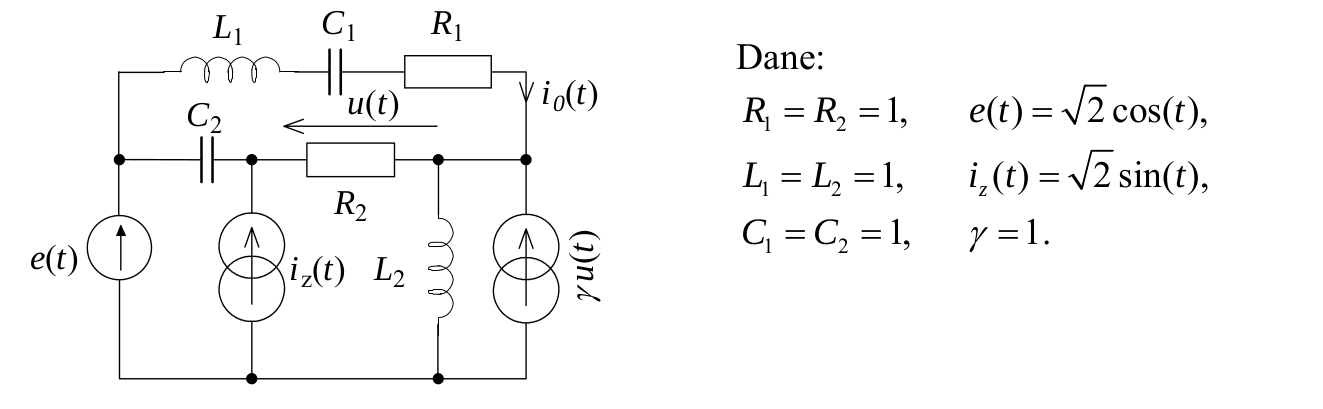
\includegraphics[width = 0.8\textwidth]{./images/Lista_3/Zadanie_2.png}
\end{figure}
\begin{flushleft}
  \textbf{Metoda prądów oczkowych}
\end{flushleft}

Zacznijmy od zamiany poszczególnych elementów na odpowiadające im impedancje oraz
połączmy węzły, w których występuje ten sam potencjał.
\begin{figure}[H]
  \centering
  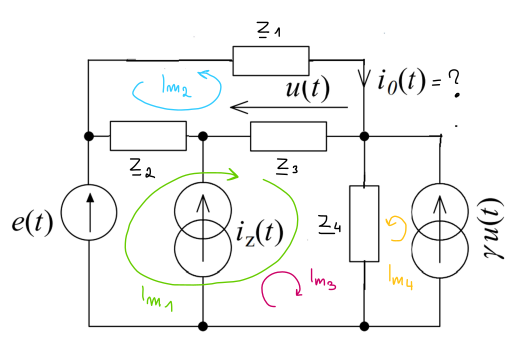
\includegraphics[width = 0.45\textwidth]{./images/Lista_3/3.2.3_MPO.png}
\end{figure}
\noindent
W następnym kroku trzeba wyliczyć wszystkie impedancje oraz zamienić napięcia
i natężenia na wskazy zespolone.
\begin{equation*}
  \underline{Z}_1 = R_1 + j\omega L_1 + \frac{1}{j\omega C_1} = 1+j-j=1
\end{equation*}
\begin{equation*}
  \underline{Z}_2 = \frac{1}{j\omega C_2} = -j
\end{equation*}
\begin{equation*}
  \underline{Z}_3 = R_2=1
\end{equation*}
\begin{equation*}
  \underline{Z}_4 = j\omega L_2 = j
\end{equation*}
\begin{equation*}
  \underline{E} = \frac{\sqrt{2}}{\sqrt{2}}j = j, \quad \omega = 1
\end{equation*}
\begin{equation*}
  \underline{I}_Z = \frac{\sqrt{2}}{\sqrt{2}} = 1, \quad \omega = 1
\end{equation*}
\begin{equation*}
  \gamma = 1
\end{equation*}

Zapiszmy więc teraz równania pomocnicze
\begin{equation*}
  \left\{
  \begin{array}{rl}
    \underline{I}_{m3} = & \underline{I}_Z                                                                              \\
    \underline{I}_{m4} = & \gamma \underline{U}                                                                         \\
    \underline{U} =      & \underline{Z}_3 \cdot \left(\underline{I}_{m1}+ \underline{I}_{m2}+\underline{I}_{m3}\right)
  \end{array}
  \right.
\end{equation*}
Kolejnym krokiem są równania zasadnicze, które pozwolą nam wyliczyć upragnione
wartości
\begin{equation}\label{3.2o_zasadnicze}
  \left\{
  \begin{array}{rl}
    \underline{E} = & \underline{I}_{m1}(\underline{Z}_2+\underline{Z}_3+\underline{Z}_4) +\underline{I}_{m2}(\underline{Z}_2+\underline{Z}_3) +\underline{I}_{m3}(\underline{Z}_3+\underline{Z}_4) +\underline{I}_{m4}\underline{Z}_4 \\
    0 =             & \underline{I}_{m1}(\underline{Z}_2+\underline{Z}_3) +\underline{I}_{m2}(\underline{Z}_1+\underline{Z}_2+\underline{Z}_3) +\underline{I}_{m3}\underline{Z}_3                                                      \\
  \end{array}
  \right.
\end{equation}

Wstawiając odpowiednie wartości do równań pomocniczych możemy wyprowadzić wzory
na wartość $\underline{I}_{m3}$ oraz $\underline{I}_{m4}$
\begin{equation*}
  \underline{I}_{m3} = 1, \quad \underline{I}_{m4} = \underline{I}_{m1} +
  \underline{I}_{m2} + 1.
\end{equation*}
Wyliczone impedancje na samym początku oraz prądy $\underline{I}_{m3}$ i
$\underline{I}_{m4}$ wstawiamy teraz do układu równań \ref{3.2o_zasadnicze}
(równań zasadniczych) co pozawala nam ułożyć układ równań \ref{3.2o_początkowe_zasadnicze}.
\begin{equation}\label{3.2o_początkowe_zasadnicze}
  \left\{
  \begin{array}{rl}
    j = & \underline{I}_{m1} + \underline{I}_{m2}(1-j)+1\cdot(1+j)+j(\underline{I}_{m1}+\underline{I}_{m2}+1) \\
    0 = & \underline{I}_{m1}(1-j)+\underline{I}_{m2}(2-j)+1                                                   \\
  \end{array}
  \right.
\end{equation}
Wykonując odpowiednie przekształcenia dojdziemy do układu równań postaci
\ref{3.2o_końcowe_zasadnicze}.
\begin{equation*}
  \left\{
  \begin{array}{rl}
    -(1+j) = & 2\cdot\underline{I}_{m1}+(1+j)(2-j)\cdot\underline{I}_{m2} \\
    -(1+j) = & (1+j)\cdot\underline{I}_{m1} + \underline{I}_{m2}          \\
  \end{array}
  \right.
\end{equation*}

\begin{equation}\label{3.2o_końcowe_zasadnicze}
  \left\{
  \begin{array}{rl}
    -(1+j) =      & 2\cdot\underline{I}_{m1} + (3+j)\underline{I}_{m2} \\
    -(1+j)(1-j) = & 2\cdot\underline{I}_{m1} + (1-j)\underline{I}_{m2} \\
  \end{array}
  \right.
\end{equation}
Odejmując stronami układ równań \ref{3.2o_końcowe_zasadnicze} pozbywamy się
niepotrzebnej zmiennej $\underline{I}_{m1}$
\begin{equation*}
  -1-j+2 = (3+j-1+j)\cdot\underline{I}_{m2},
\end{equation*}
co pozwala nam wyliczyć wartość zespoloną $\underline{I}_{m2}$
\begin{equation*}
  \underline{I}_{m2} = \frac{1-j}{2+2j} = \frac{1}{4}(1-j)^2 = -\frac{1}{2}j.
\end{equation*}
Ze względu, że $\underline{I}_{m2}$ jest przeciwnie skierowane do $\underline{I}_0$,
musimy wziąć przeciwną wartość co daje nam taki wynik
\begin{equation*}
  \underline{I}_0 = - \underline{I}_{m2} = \frac{1}{2}j.
\end{equation*}

Na koniec wystarczy zamienić wyrażenie z postaci algebraicznej na postać sinusoidalną,
co daje nam wynik końcowy
\begin{equation*}
  i_0(t) = \frac{\sqrt{2}}{2}\cos(t)\; A.
\end{equation*}

\begin{flushleft}
  \textbf{Metoda potencjałów węzłowych}
\end{flushleft}

Tak jak w metodzie prądów oczkowych, na początku połączmy węzły, które mają
ten sam potencjał, jednak tym razem zamiast impedancji wyznaczamy admitancję
poszczególnych elementów.
\begin{figure}[H]
  \centering
  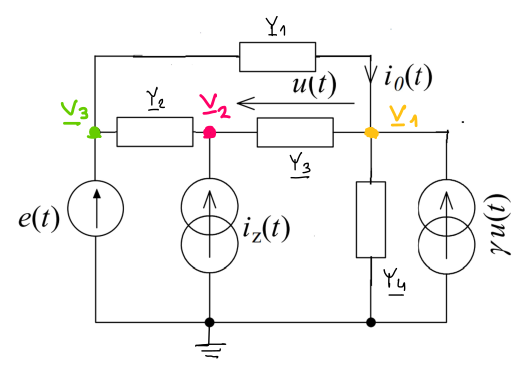
\includegraphics[width = 0.45\textwidth]{./images/Lista_3/3.2.3_MPV.png}
\end{figure}

\begin{equation*}
  \underline{Y}_1 = \frac{1}{\underline{Z}_1} = 1, \quad \underline{Y}_2 = \frac{1}{\underline{Z}_2} = j
\end{equation*}
\begin{equation*}
  \underline{Y}_3 = \frac{1}{\underline{Z}_3} = 1, \quad \underline{Y}_4 = \frac{1}{\underline{Z}_4} = -j
\end{equation*}
\begin{equation*}
  \underline{E} = j, \quad \omega = 1
\end{equation*}
\begin{equation*}
  \underline{I}_Z = 1, \quad \omega = 1
\end{equation*}
\begin{equation*}
  \gamma = 1
\end{equation*}

Zapiszmy więc teraz równania pomocnicze
\begin{equation*}
  \left\{
  \begin{array}{rl}
    \underline{V}_3 = & \underline{E}                      \\
    \underline{U} =   & \underline{V}_2 - \underline{V}_1,
  \end{array}
  \right.
\end{equation*}
a następnie równania zasadnicze
\begin{equation}\label{3.2v_zasadnicze}
  \left\{
  \begin{array}{rl}
    \gamma\cdot\underline{U} = & \underline{V}_1 \left(\underline{Y}_1+\underline{Y}_3+\underline{Y}_4\right)-\underline{V}_2\underline{Y}_3-\underline{V}_3\underline{Y}_1 \\
    \underline{I}_Z =          & - \underline{V}_1\underline{Y}_3 + \underline{V}_2\left(\underline{Y}_2+\underline{Y}_3\right) -\underline{V}_3\underline{Y}_2.
  \end{array}
  \right.
\end{equation}
Wstawiając odpowiednie wartości do równań pomocniczych możemy wyznaczyć
$\underline{V}_3$
\begin{equation*}
  \underline{V}_3 = j, \quad \underline{U} = \underline{V}_2 - \underline{V}_1.
\end{equation*}
Wstawiając teraz te wartości do układu równań \ref{3.2v_zasadnicze} (równań
zasadniczych) otrzymujemy układ dwóch równań z tylko dwoma niewiadomymi
\begin{equation*}
  \left\{
  \begin{array}{rl}
    \underline{V}_2 - \underline{V}_1 = & \underline{V}_1(2-j) - \underline{V}_2 -j           \\
    1 =                                 & - \underline{V}_1 + \underline{V}_2(1+j) -j\cdot j.
  \end{array}
  \right.
\end{equation*}
Wykonując dalsze przekształcenia otrzymamy układ równań \ref{3.2v_końcowe_zasadnicze}.
\begin{equation*}
  \left\{
  \begin{array}{rl}
    j = & \underline{V}_1 (3-j)- 2\underline{V}_2 \\
    0 = & -\underline{V}_1 + \underline{V}_2(1+j)
  \end{array}
  \right.
\end{equation*}

\begin{equation}\label{3.2v_końcowe_zasadnicze}
  \left\{
  \begin{array}{rl}
    j = & \underline{V}_1(3-j) - 2\underline{V}_2  \\
    0 = & -(1-j)\underline{V}_1 + 2\underline{V}_2
  \end{array}
  \right.
\end{equation}

Odejmując stronami równania \ref{3.2v_końcowe_zasadnicze} pozbywamy się
niepotrzebnego składnika $\underline{V}_2$, co pozwoli nam wyliczyć $\underline{V}_1$.
\begin{equation*}
  j = (3-j-1+j)\underline{V}_1
\end{equation*}
\begin{equation*}
  \underline{V}_1 = \frac{1}{2}j
\end{equation*}

Na koniec wystarczy obliczyć $\underline{I}_0$
\begin{equation*}
  \underline{I}_0 = \underline{Y}_1(\underline{V}_3-\underline{V}_1) =
  j - \frac{1}{2}j = \frac{1}{2}j,
\end{equation*}
co pozwoli zapisać końcowy wynik
\begin{equation*}
  i_0(t) = \frac{\sqrt{2}}{2}\cos(t)\; A.
\end{equation*}

\subsection{Zadanie 3}
\textbf{Obliczyć prąd $i_0(t)$ za pomocą tw. Thevenina.}
\begin{figure}[H]
  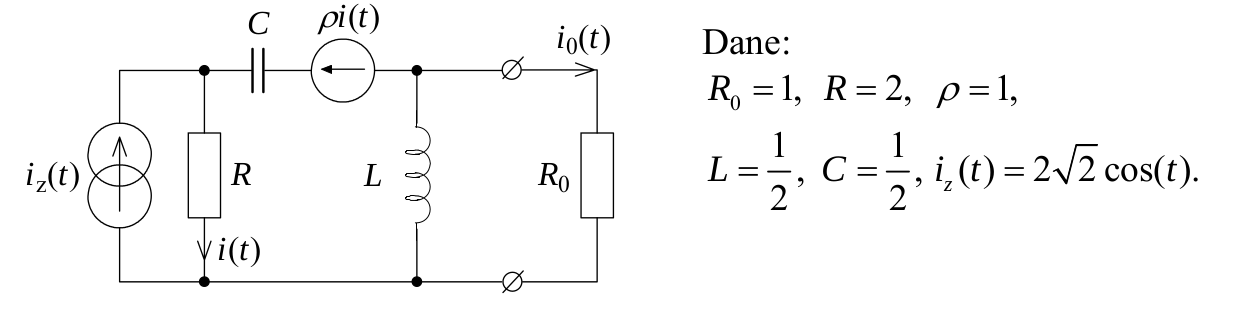
\includegraphics[width = 0.8\textwidth]{./images/Lista_3/Zadanie_3.png}
\end{figure}

\begin{figure}[H]
  \centering
  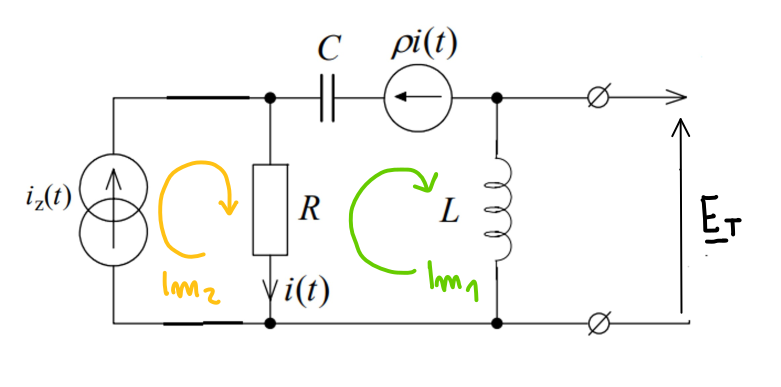
\includegraphics[width = 0.5\textwidth]{./images/Lista_3/3.3.1.png}
\end{figure}
\noindent
\textit{Zmienione dane, aby się wygodniej liczyło:}
\begin{equation*}
  R = 2, \quad C = 2, \quad L = \frac{1}{2}, \quad \rho = 1
\end{equation*}

Zapiszmy na początek nasz prąd $i_Z(t)$ jako wskaz zespolony
\begin{equation*}
  \underline{I}_Z = \frac{2\sqrt{2}}{\sqrt{2}}j = 2j, \quad \omega = 1.
\end{equation*}
Wyznaczamy teraz równania pomocnicze, z których jedno zawiera prąd $\underline{I}$,
sterujący rzeczywistym źródłem napięcia
\begin{equation*}
  \underline{I} = \underline{I}_{m2} - \underline{I}_{m1},
\end{equation*}
\begin{equation*}
  \underline{I}_{m2} = \underline{I}_Z.
\end{equation*}

Napiszmy teraz równanie dla oczka $\underline{I}$, pamiętając o odpowiednich zwrotach
\begin{equation}\label{3.3_oczko_Im1}
  -\rho\underline{I} = \underline{I}_{m1}\left(R+j\omega L+\frac{1}{j\omega C}\right)
  - \underline{I}_{m2} R.
\end{equation}
Wstawiając odpowiednie wartości do równań pomocniczych
\begin{equation*}
  \underline{I}_{m2} = 2j \quad \Rightarrow \quad \underline{I} = 2j - \underline{I}_{m1},
\end{equation*}
a następnie te wartości do równania \ref{3.3_oczko_Im1}
\begin{equation*}
  \underline{I_{m1}} - 2j = \underline{I}_{m1} \cdot 2 - 4j,
\end{equation*}
możemy wyliczyć prąd $\underline{I_{m1}}$
\begin{equation*}
  \underline{I_{m1}} = 2j.
\end{equation*}
Mnożąc prąd $\underline{I}_{m1}$ poprzez impedancję na induktorze $L$ otrzymujemy
spadek napięcia $\underline{E_T}$
\begin{equation*}
  \underline{E_T} = j\omega L\cdot\underline{I_{m1}} = \frac{1}{2}j\cdot 2j = -1.
\end{equation*}

Skoro mamy już napięcie Thevenina, teraz trzeba policzyć impedancję zastępczą.
Zgodnie z zasadą rozwieramy źródło pobudzające. Musimy przez to dołączyć
źródło napięcia, ponieważ źródło sterowane nie może być pobudzeniem.
\begin{figure}[H]
  \centering
  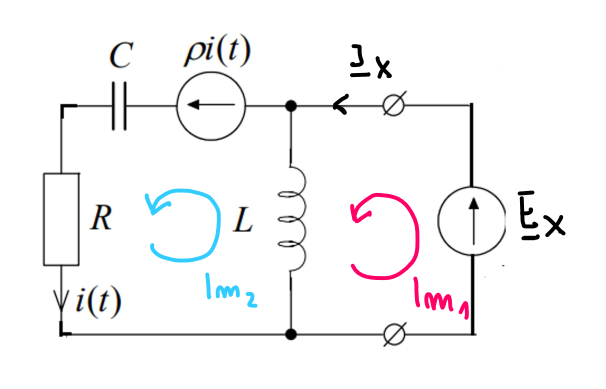
\includegraphics[width = 0.4\textwidth]{./images/Lista_3/3.3.2.png}
\end{figure}
Na początku piszemy wzór na impedancję zastępczą
\begin{equation*}
  \underline{Z}_g = \frac{\underline{E}_x}{\underline{I}_x}.
\end{equation*}
W następnym korku powinniśmy napisać równanie pomocnicze
\begin{equation}\label{3.3_2_pomocnicze}
  \underline{I} =   \underline{I}_{m2}
\end{equation}
oraz równania zasadnicze
\begin{equation}\label{3.3_2_zasadnicze}
  \left\{
  \begin{array}{rl}
    \underline{E}_x =    & \underline{I}_{m1}\cdot j\omega L -\underline{I}_{m2} \cdot j\omega L                                  \\
    \rho \underline{I} = & -\underline{I}_{m1}\cdot j\omega L + \underline{I}_{m2}\left(R+j\omega L + \frac{1}{j\omega C}\right).
  \end{array}
  \right.
\end{equation}
Pomocne również będzie mieć w pamięci, że $\underline{I}_x = \underline{I}_{m1}$.

Wstawiając teraz do równania \ref{3.3_2_zasadnicze} elementy z równania
\ref{3.3_2_pomocnicze} oraz wykonaniu odpowiednich przekształceń otrzymamy układ równań postaci
\ref{3.3_2_zasadnicze_końcowe}.
\begin{equation*}
  \left\{
  \begin{array}{rl}
    \underline{E}_x = & \frac{1}{2}j\cdot\underline{I}_{m1}- \frac{1}{2}j\cdot\underline{I}_{m2} \\
    0 =               & -\frac{1}{2}j\cdot\underline{I}_{m1} + \underline{I}_{m2}                \\
  \end{array}
  \right.
\end{equation*}
\begin{equation}\label{3.3_2_zasadnicze_końcowe}
  \left\{
  \begin{array}{rl}
    -2j\cdot\underline{E}_x = & \underline{I}_{m1}-\underline{I}_{m2}                     \\
    0 =                       & -\frac{1}{2}j\cdot\underline{I}_{m1} + \underline{I}_{m2} \\
  \end{array}
  \right.
\end{equation}
Po dodaniu stronami równań \ref{3.3_2_zasadnicze_końcowe} pozbędziemy się składnika
$\underline{I}_{m2}$
\begin{equation*}
  -2j\cdot\underline{E}_x = \left(1-\frac{1}{2}j\right)\cdot\underline{I}_{m1},
\end{equation*}
co pozwoli nam wyliczyć impedancję zastępczą $\underline{Z}_g$
\begin{equation*}
  \underline{Z}_g = \frac{\underline{E}_x}{\underline{I}_x} = \frac{1-\frac{1}{2}j}{-2j}
  = \frac{1}{4} + \frac{1}{2}j.
\end{equation*}


\begin{figure}[H]
  \begin{flushleft}
    Na koniec do naszego zastępczego dwójnika dołączamy rezystor $R_0$ i obliczamy
    zespolony prąd $\underline{I}_0$.
  \end{flushleft}
  \centering
  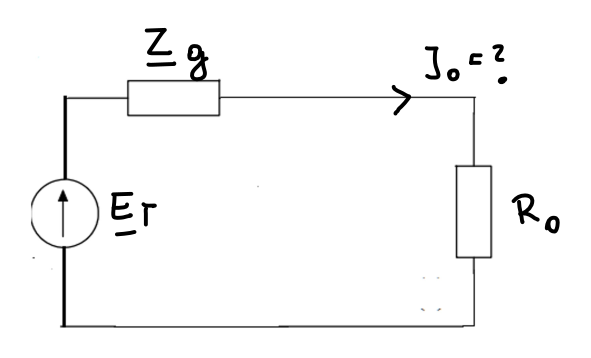
\includegraphics[width = 0.4\textwidth]{./images/Lista_3/3.3.3.png}
\end{figure}

Zgodnie z metodą prądów oczkowych prąd $\underline{I}_0$ będzie określony wzorem
\begin{equation}\label{3.3_3_i0}
  \underline{I}_0 = \frac{\underline{E}_T}{R_0 + \underline{Z}_g}.
\end{equation}
Wstawiając teraz odpowiednie wartości do równania \ref{3.3_3_i0} możemy wyliczyć
wartość prądu $\underline{I}_0$ w postaci algebraicznej
\begin{equation*}
  \underline{I}_0 = \frac{-1}{1 + \frac{1}{4} + \frac{1}{2}j} = -\frac{4}{29}(5-2j),
\end{equation*}
a następnie przekształcić ją do postaci wykładniczej
\begin{equation*}
  \underline{I}_0 = -\frac{4}{29}\sqrt{29}e^{-j\arc \tan \frac{2}{5}},
\end{equation*}
co pozwoli zapisać nam końcowy wynik w postaci sinusoidalnej
\begin{equation*}
  i_0(t) = -\frac{4}{29}\sqrt{29}\sqrt{2}\sin\left(t-\arc\tan\frac{2}{5}\right).
\end{equation*}
\begin{equation*}
  i_0(t) = \frac{4}{29}\sqrt{29}\sqrt{2}\sin\left(t+\pi-\arc\tan\frac{2}{5}\right)
\end{equation*}

\subsection{Zadanie 4}
\textbf{Wyznaczyć prąd $i(t)$ w stanie ustalonym.}
\begin{figure}[H]
  \centering
  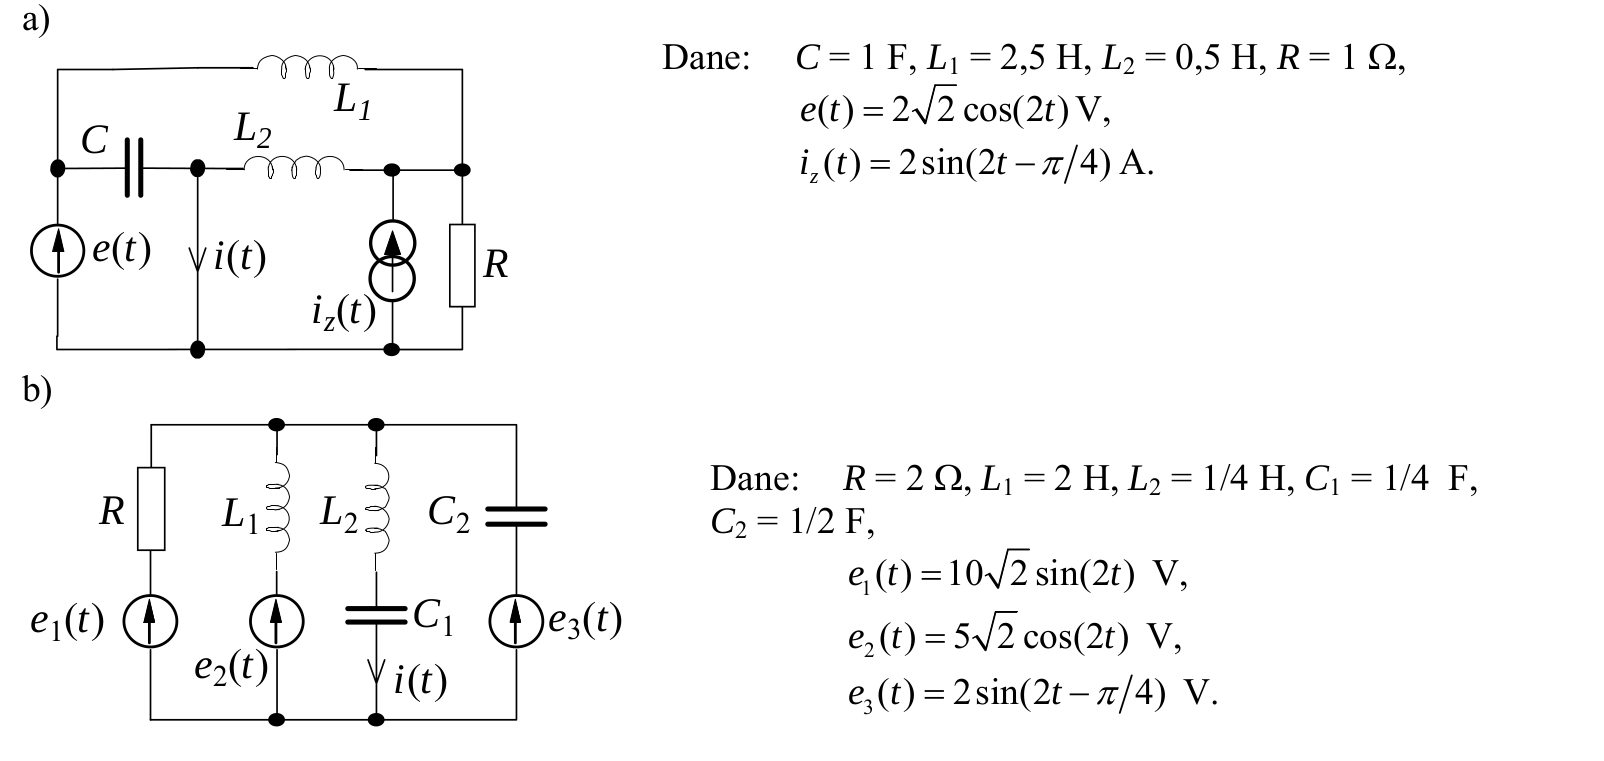
\includegraphics[width = \textwidth]{./images/Lista_3/Zadanie_4.png}
\end{figure}

\begin{enumerate}[label=\alph*)]
  \item Przerysujmy na początek ten układ w taki sposób, który ułatwi nam identyfikację
        napięć na poszczególnych węzłach układu.
        \begin{figure}[H]
          \centering
          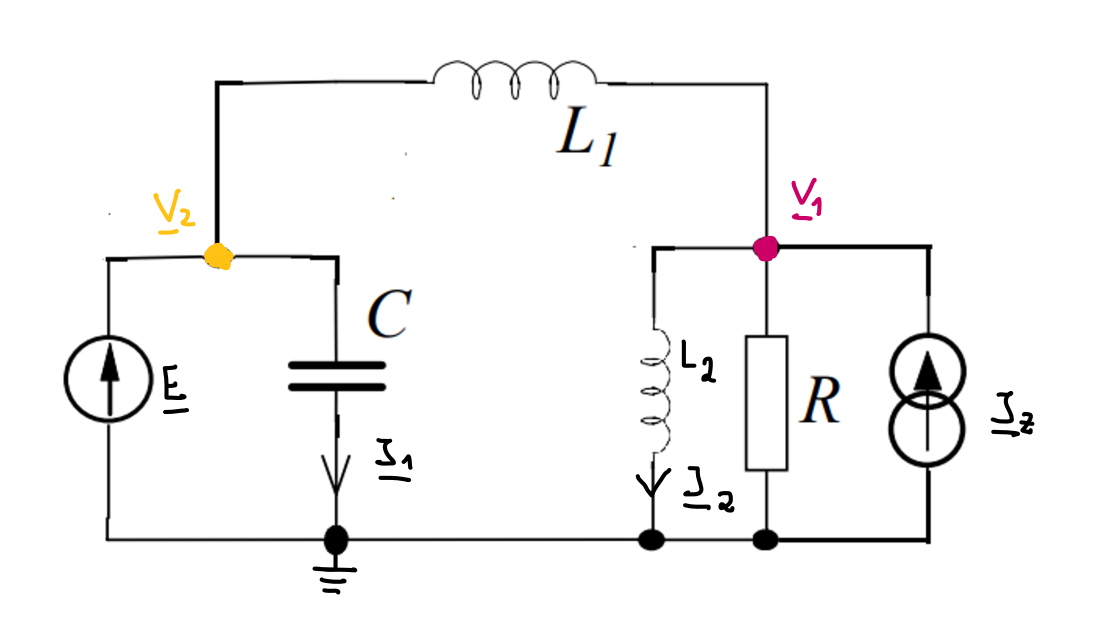
\includegraphics[width = 0.5\textwidth]{./images/Lista_3/3.4.1.png}
        \end{figure}
        Na początku jak zawsze zamieńmy postać sinusoidalną napięcia $e(t)$
        \begin{equation*}
          e(t) = 4\cos(2t-45^\circ),
        \end{equation*}
        na algebraiczną
        \begin{equation*}
          \underline{E} = \frac{4}{\sqrt{2}}\left(\frac{1}{\sqrt{2}}-
          \frac{1}{\sqrt{2}}j\right)j = 2+2j, \quad \omega = 2.
        \end{equation*}
        Tak samo musimy postąpić z prądem $i_Z(t)$
        \begin{equation*}
          i_Z(t) = 2\sin(2t+45^\circ),
        \end{equation*}
        \begin{equation*}
          \underline{I} = \frac{2}{\sqrt{2}}\left(\frac{1}{\sqrt{2}}+
          \frac{1}{\sqrt{2}}j\right) = 1 + j, \quad \omega = 2.
        \end{equation*}
        \textit{Zmienione dane, aby się wygodniej liczyło:}
        \begin{equation*}
          L_1 = 1, \quad L_2 = \frac{1}{3}, \quad R = \frac{1}{2}, \quad
          C = \frac{3}{16}
        \end{equation*}
        Jak widać z przerysowanego obwodu wartość $V_2$ będzie równa wartości $\underline{E}$
        co pozwala zapisać takie równanie
        \begin{equation}\label{3.4a_V2}
          \underline{V}_2 = \underline{E}.
        \end{equation}
        \textit{\textcolor{Red}{Tutaj jeszcze nie wiem skąd to się wzięło}}
        \begin{equation}\label{3.4_IZ}
          \underline{I}_Z = \underline{V}_1 \left(\frac{1}{R}+
          \frac{1}{j\omega L_1}+\frac{1}{j\omega L_2}\right) - \underline{V}_2
          \frac{1}{j\omega L_1}
        \end{equation}
        Przekształcając równanie \ref{3.4_IZ} oraz wstawiając do niego równianie \ref{3.4a_V2}
        otrzymujemy wzór końcowy na wyliczenie wartości $V_1$
        \begin{equation*}
          \underline{V}_1 = \frac{\underline{I}_Z+\dfrac{\underline{E}}{j\omega L_1}}
          {\dfrac{1}{R}+\dfrac{1}{j\omega L_1}+\dfrac{1}{j\omega L_2}},
        \end{equation*}
        a wstawiając do niego odpowiednie wartości otrzymujemy wartość napięcia zespolonego
        $V_1$
        \begin{equation*}
          \underline{V}_1 = \frac{1+j-\dfrac{1}{2}j\cdot2(1+j)}
          {2-\dfrac{1}{2}j-\dfrac{3}{2}j} = \frac{(1+j)(1-j)}{2-2j} = \frac{1}{1-j}
          = \frac{1}{2}(1+j).
        \end{equation*}
        Prąd końcowy jak widać na przerysowanym obwodzie będzie sumą prądów
        $\underline{I}_1$ oraz $\underline{I}_2$, co pozwala nam zapisać taki wzór
        \begin{equation*}
          \underline{I} = j\omega C\underline{E} + \frac{\underline{V}_1}{j\omega L_2},
        \end{equation*}
        a wstawiając do niego odpowiednie wartości możemy wyliczyć zespolony prąd
        $\underline{I}$
        \begin{equation*}
          \underline{I} = j\frac{3}{8}\cdot2(1+j)-j\frac{3}{2}\cdot\frac{1}{2}
          (1+j) = (1+j)\left(j\frac{3}{4}-j\frac{3}{4}\right) = 0.
        \end{equation*}
        Jak widać prąd w stanie ustalonym będzie wynosił $0$ więc możemy zapisać
        odpowiedź końcową
        \begin{equation*}
          i(t) = 0.
        \end{equation*}
  \item Przerysujmy na początek ten układ do postaci, w której rzeczywiste źródła
        napięcia będą się znajdowały obok siebie,
        \begin{figure}[H]
          \centering
          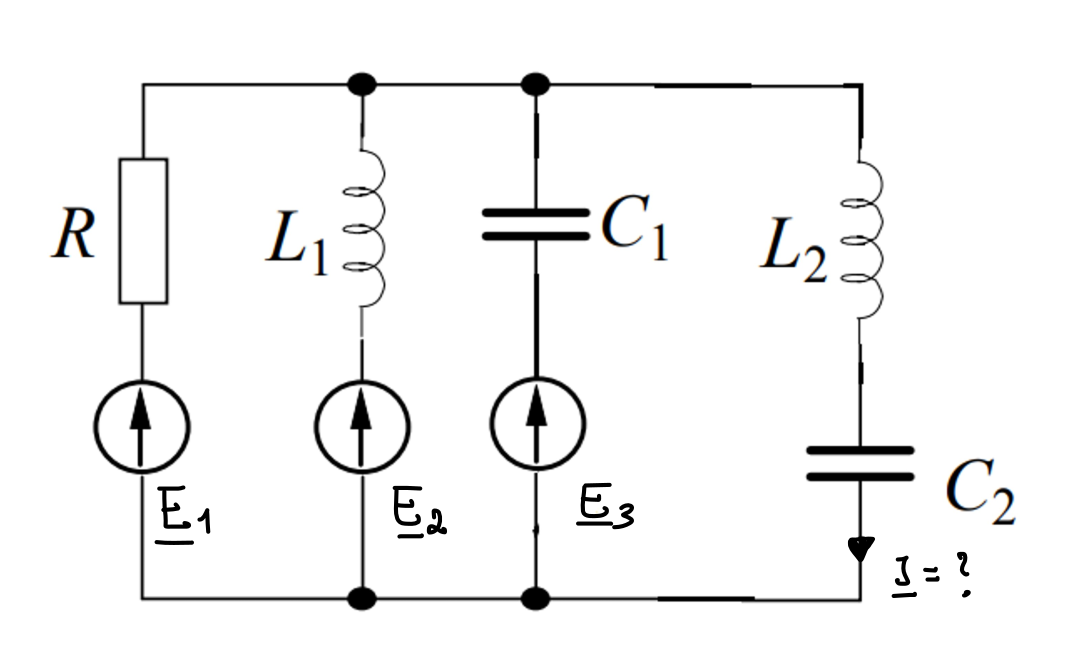
\includegraphics[width = 0.5\textwidth]{./images/Lista_3/3.4.2.png}
        \end{figure}
        a następnie wszystkie wartości źródeł napięciowych zamieńmy z postaci sinusoidalnej,
        na postać algebraiczną.
        \begin{equation*}
          e_1(t) = 10\sqrt{2}\sin(2t) \quad \Rightarrow \quad
          \underline{E}_1 = 10\frac{\sqrt{2}}{\sqrt{2}} = 10, \: \omega = 2
        \end{equation*}
        \begin{equation*}
          e_2(t) = 6\sqrt{2}\cos(2t) \quad \Rightarrow \quad
          \underline{E}_2 = 6\frac{\sqrt{2}}{\sqrt{2}}j = 6j, \: \omega = 2
        \end{equation*}
        \begin{equation*}
          e_3(t) = 2\sin\left(2t-\frac{\pi}{4}\right) \quad \Rightarrow \quad
          \underline{E}_3 = \frac{2}{\sqrt{2}}e^{-j\frac{\pi}{4}} = 1-j, \: \omega = 2
        \end{equation*}
        \textit{Zmienione dane, aby się wygodniej liczyło:}
        \begin{equation*}
          R = 5, \quad L_1 = 1, \quad C_1 = \frac{1}{2}, \quad L_2 = \frac{1}{2},
          \quad C_2 = \frac{1}{2}.
        \end{equation*}
        Połączmy induktor $L_2$ i kondensator $C_2$ w jedną impedancję
        \begin{equation*}
          \underline{Z}_1 = j\omega L_2 + \frac{1}{j\omega C_2} = j-j = 0.
        \end{equation*}
        Przerysujmy teraz układ zamieniając rzeczywiste źródła napięcia na rzeczywiste
        źródła prądowe.
        \begin{figure}[H]
          \centering
          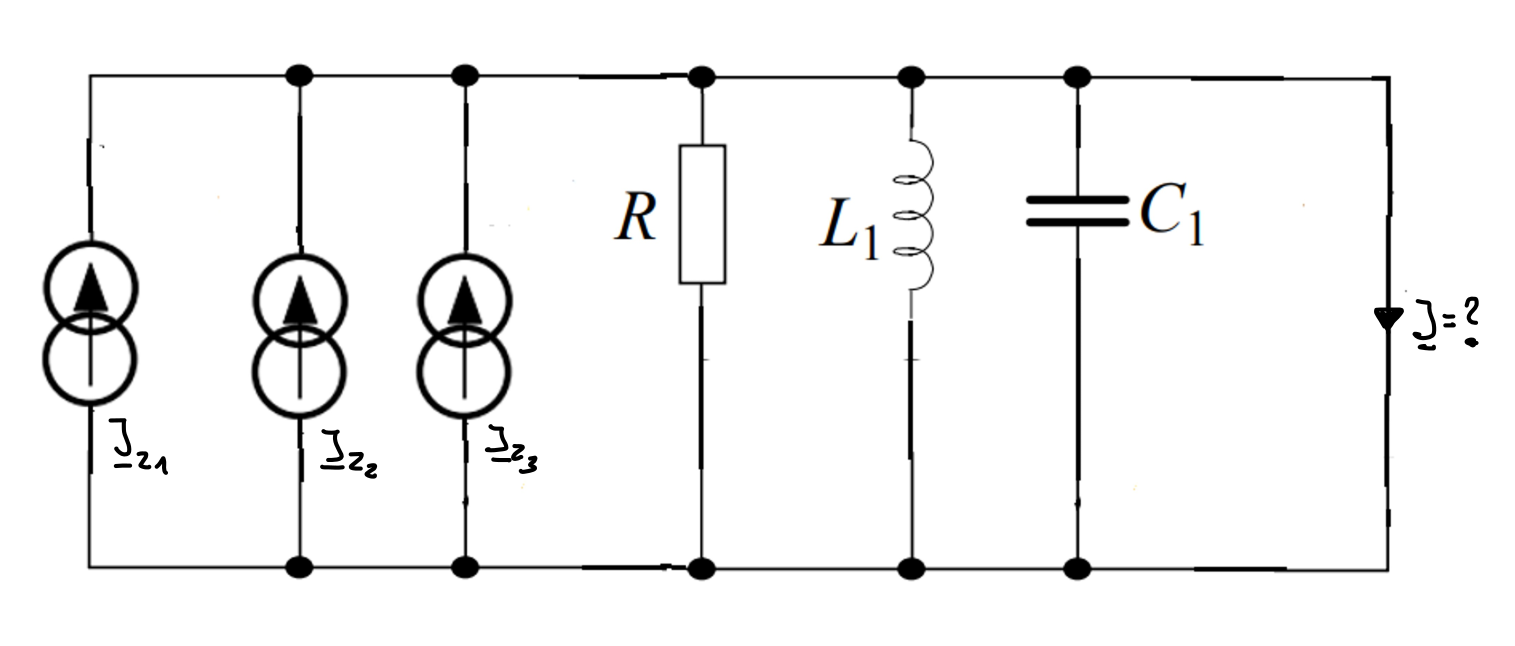
\includegraphics[width = 0.6\textwidth]{./images/Lista_3/3.4.3.png}
        \end{figure}
        Ze względu na to, że impedancja $Z_1$ wynosi zero to w obwodzie już nie musimy jej
        uwzględniać. Policzmy więc wartości tych natężeń zespolonych.
        \begin{equation*}
          \underline{I}_{Z1} = \frac{\underline{E}_1}{R_1} = \frac{10}{5} = 2
        \end{equation*}
        \begin{equation*}
          \underline{I}_{Z2} = \frac{\underline{E}_2}{j\omega L_1} = \frac{6j}
          {j\cdot2\cdot1} = 3
        \end{equation*}
        \begin{equation*}
          \underline{I}_{Z3} = j\omega C_1\cdot\underline{E}_3 = j(1-j) = 1+j
        \end{equation*}
        Możemy teraz wyprowadzić równanie na całkowity prąd zespolony
        \begin{equation}\label{3.4b_prad}
          \underline{I} = \underline{I}_{Z1} + \underline{I}_{Z2} + \underline{I}_{Z3}.
        \end{equation}
        Wstawiając wartości poszczególnych prądów zespolonych do równania \ref{3.4b_prad}
        możemy wyliczyć prąd zespolony w stanie ustalonym. Wynik ten od razu możemy przedstawić
        w postaci wykładniczej
        \begin{equation*}
          \underline{I} =2+3+1+j = 6 + j = \sqrt{37}e^{j\arc \ctg\left(
          \dfrac{1}{6}\right)},
        \end{equation*}
        co pozwoli nam zapisać wynik końcowy w postaci sinusoidalnej
        \begin{equation*}
          i(t) = \sqrt{37}\sqrt{2}\sin\left(2t+\arc \ctg\left(\dfrac{1}{6}\right)\right)\; A,
        \end{equation*}
        \begin{equation*}
          i(t) = 8,602\sin\left(2t+9,46^\circ\right)\; A.
        \end{equation*}
\end{enumerate}

\section{Lista 4}
\subsection{Zadanie 1}
\textbf{Narysować następujące funkcje oraz wyznaczyć ich transformaty Laplace’a:}
\begin{enumerate}[label=\alph*)]
  \item $e^{-2t} 1(t)$,
  \item $e^{-2(t-1)} 1(t)$,
  \item $e^{-2t} 1(t-1)$,
  \item $e^{-2(t-1)} 1(t-1)$.
\end{enumerate}

\subsection{Zadanie 2}
\textbf{Wyznaczyć transformaty Laplace’a następujących funkcji:}
\begin{figure}[H]
  \centering
  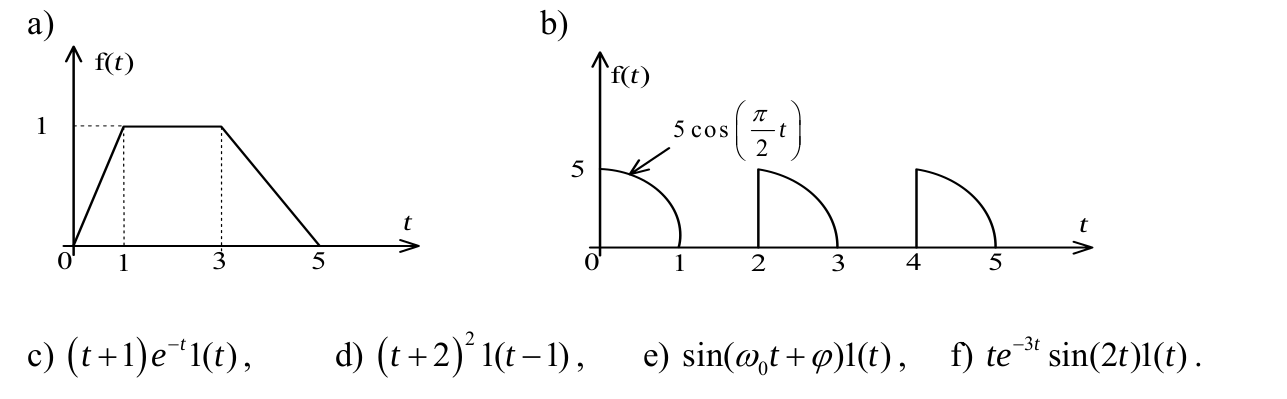
\includegraphics[width = \textwidth]{./images/Lista_4/Zadanie_2.png}
\end{figure}

\subsection{Zadanie 3}
\textbf{Wyznaczyć odwrotne transformaty Laplace’a następujących funkcji:}
\begin{figure}[H]
  \centering
  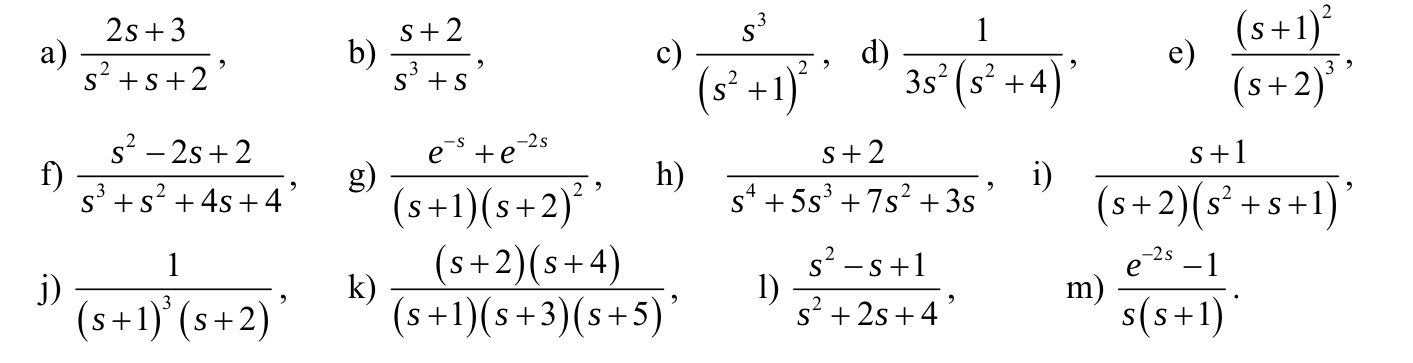
\includegraphics[width = \textwidth]{./images/Lista_4/Zadanie_3.png}
\end{figure}

\subsection{Zadanie 4}
\textbf{Wyznaczyć składową przejściową i ustaloną, jeżeli klucz K zwarto w chwili t=0.
  Warunki początkowe są zerowe.}
\begin{figure}[H]
  \centering
  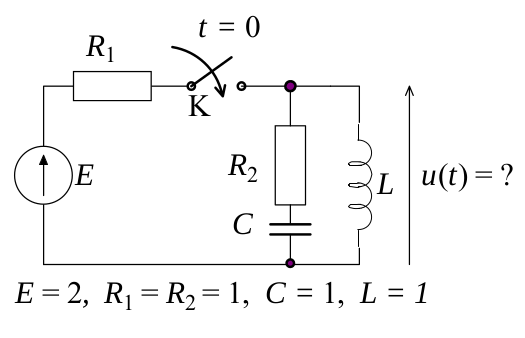
\includegraphics[width = 0.5\textwidth]{./images/Lista_4/Zadanie_4.png}
\end{figure}

\subsection{Zadanie 5}
\textbf{W obwodzie występował stan ustalony. W chwili t=0 klucz K zwarto. Wyznaczyć
  napięcie $u_C(t)$ dla t $\geq$ 0.}
\begin{figure}[H]
  \centering
  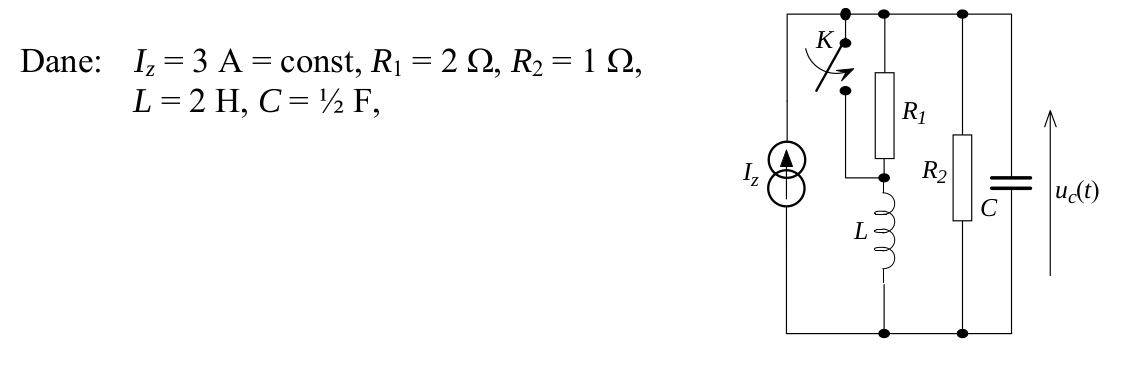
\includegraphics[width = \textwidth]{./images/Lista_4/Zadanie_5.png}
\end{figure}

\subsection{Zadanie 6}
\textbf{Klucz był w pozycji 1 nieskończenie długo. W chwili t = 0 klucz przełączono w
  pozycję 2. Wyznaczyć napięcie u(t) dla t $\geq$ 0.}
\begin{figure}[H]
  \centering
  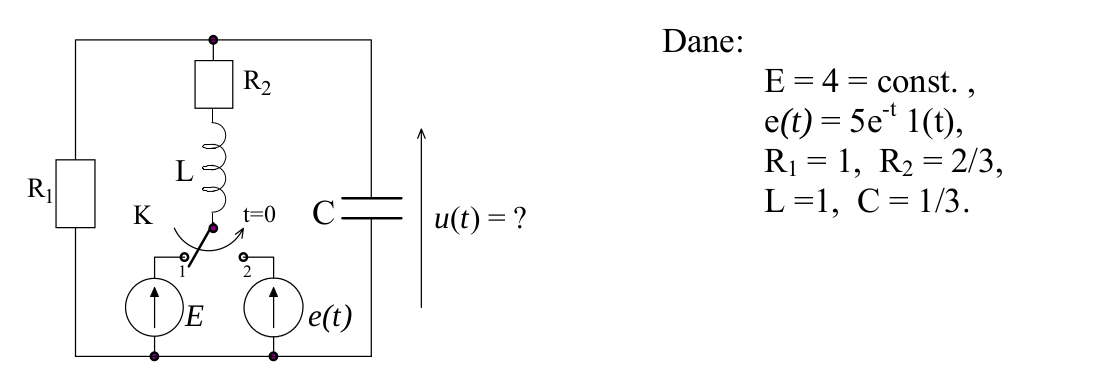
\includegraphics[width = \textwidth]{./images/Lista_4/Zadanie_6.png}
\end{figure}

\newpage
\Large{TODO:}
\begin{itemize}
  \item Rozwiązać listę 4
  \item Opisać zadanie 3.2
  \item Opisać zadanie 3.3
  \item Rozwiązać zadanie 1.6
  \item Rozwiązać zadanie 1.1
\end{itemize}
\end{document}
